\newpage
%\chapter{Results and discussion}

\section{Results and discussion}
In this section the results of the simulations will be presented and discussed. Two different variations of the LB solver were tested. One with the optimised values of the relaxation parameters~\cite{geier:parameter} and other with the relaxation parameters used as specified in ~\cite{geier:cumulant}. The results presented in this section are performed with the former variation of the LB solver and the results of the latter variation will just be presented in the Appendix (\ref{One wale}), as the choice of value one for all the parameters is the most stable choice but not accurate enough~\cite{geier:parameter}. Firstly, the results of the LB simulations carried out without any turbulence model will be presented and discussed. The result of the simulations with no-model will be termed as the \emph{under resolved DNS} (UDNS). Under resolved because the resolution is coarser compared to the reference mesh resolution and DNS because no additional modelling is done for turbulence. It will be followed by the discussion of the results from the LB-LES with the WALE model and will be compared with the UDNS and DNS results. Few general comments applicable for all the simulations are:

\begin{itemize}
\item The DNS results of~\cite{kim:moin:moser:87} , for $Re_\tau = 395$, will be used as a reference for the comparison. The quantities obtained from the DNS data will be referred to as the \emph{target} quantities.
\item The results shown here are plotted against the global coordinates, $y/\de$, and local coordinates,  $y^+$.  
\item All simulations have been performed using the single precision on GPGPUs. 
\item The normalised wall distance $y^+$ used in the profile plots is computed a posteriori for all the simulations.
%\item Since the channel flow is symmetric, the profiles have been plotted over the  
\end{itemize}

\subsection{UDNS results} \label{UDNS profiles}
To test the accuracy of the turbulent channel flow results from the LB solver, against the DNS data, these simulations have been performed. The physical quantities resulting from the simulations for all meshes are listed in the table (\ref{Global quantities}). The average friction velocity ($u_\tau$) and the $Re_\tau$ resulting from the computed $u_\tau$ are the important quantities. From now on $u_\tau$ represents the average friction velocity. The computed value of $u_\tau$ is under-predicted for all the simulations and so is the resulting $Re_\tau$, but the values approach the target $u_\tau$ with the increase in the mesh resolution. We know from the definition of $u_\tau$,that $u_\tau$ is proportional to the $\tau_w$. Thus, smaller values of the $u_\tau$ implies smaller values of $\tau_w$.  
%
\begin{table}[h!]
\begin{center}
\begin{tabular}{ p{3cm}|p{1.5cm}p{1.5cm}p{1.5cm}p{1.5cm}  } 
\hline
Physical quantity & Mesh1 & Mesh1\_5 & Mesh2 & Target \\
  \hline
  \multirow{1}{6em}{$u_\tau,\ m/s$}  & 0.0070 & 0.0074 & 0.0076 & 0.0079\\
  \hline
  \multirow{1}{6em}{$Re_\tau$} & 352 & 371 & 382 & 395\\
  \hline
  \multirow{1}{6em}{$U_c,\ m/s$} & 0.1565 & 0.1563 & 0.1557 & 0.1591\\
  \hline
\end{tabular}
\end{center}
\caption{Comparison of the resulting physical quantities}
\label{Global quantities}
\end{table}
%
\subsubsection{Mean velocity profile} \label{Mean velocity UDNS}

Mean velocity profiles presented here have been averaged in time and space. It is seen from the Fig. (\ref{mean profile udns}), the mean velocity profiles for all the meshes over-predict the DNS data. As discussed in the section \ref{scaling} the viscous sublayer plays a dominant role on the flow characteristics as higher velocity gradients are present there. Since the viscous sublayer is under-resolved in the simulations, $u_\tau$ and eventually the $\tau_w$ is under-predicted and as a result we see the different flow characteristics obtained from the simulations i.e. over-predicting velocity profiles in comparison to the DNS data. It is clear that with the better resolution of the viscous sublayer, the correct flow characteristics will be obtained and it is apparent from the Fig. (\ref{mean profile udns}) that with the mesh refinement, the velocity profiles approach closer to the DNS data. Velocity profile for mesh3 nearly collapses on to the DNS data. Thus a positive effect of mesh resolution is seen from the mean velocity profile plots. 
%
%
\begin{figure}[h]
%\centering
\begin{minipage}[b]{0.5\textwidth}
\subfigure[global coordinates]{
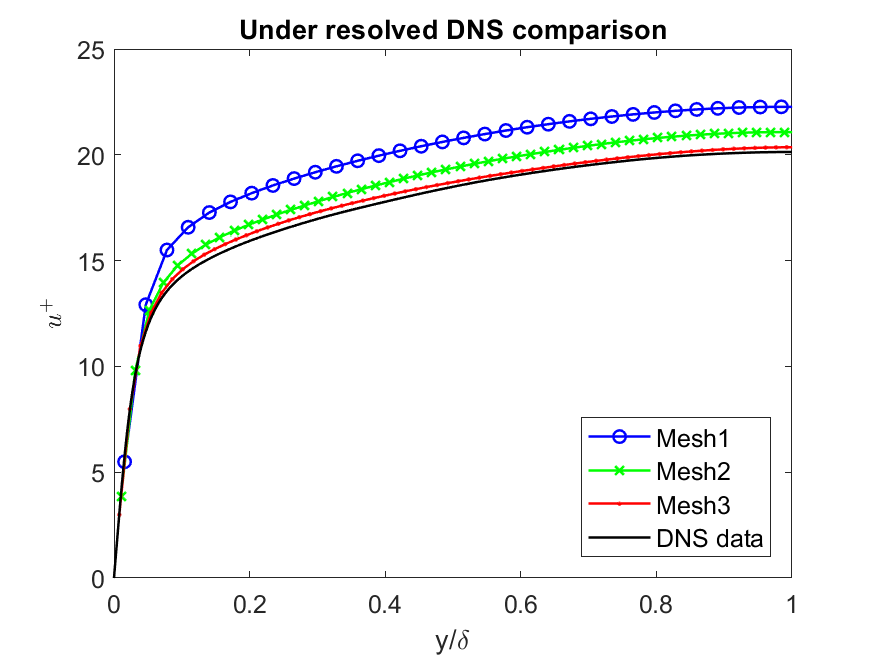
\includegraphics[width=6.7cm]{06_Resultsanddiscussion/figur/UDNS_2016/Profile_global_coords.png}}
\end{minipage}
%
\begin{minipage}[b]{0.5\textwidth}
\subfigure[wall coordinates]{
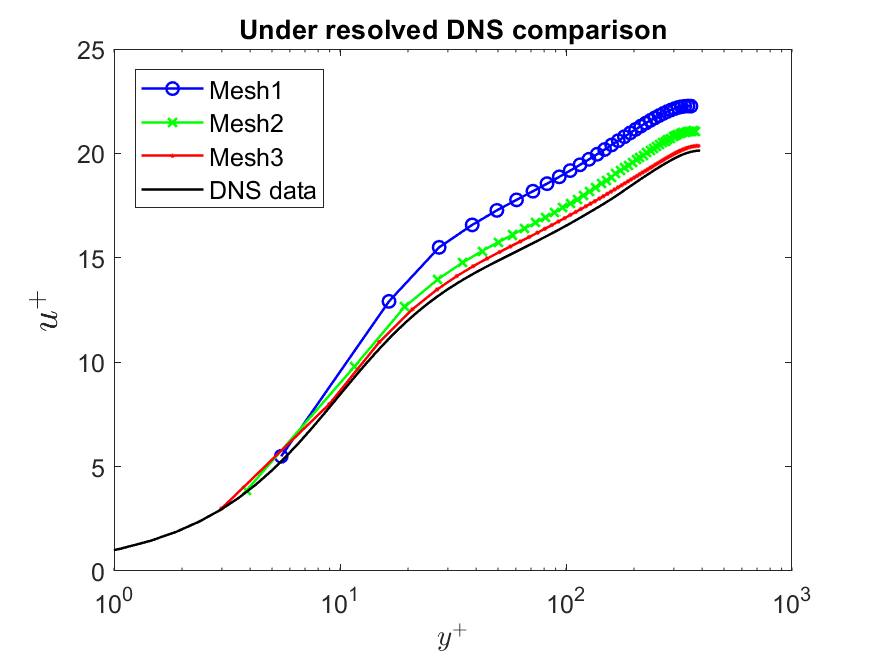
\includegraphics[width=6.7cm]{06_Resultsanddiscussion/figur/UDNS_2016/Profile_wall_coords_theo_comp.png}}
\end{minipage}
\caption{Mean stream-wise velocity profile normalized by $u_\tau$}
\label{mean profile udns}
\end{figure}
%
%\begin{figure}[h]
%    \centering
%    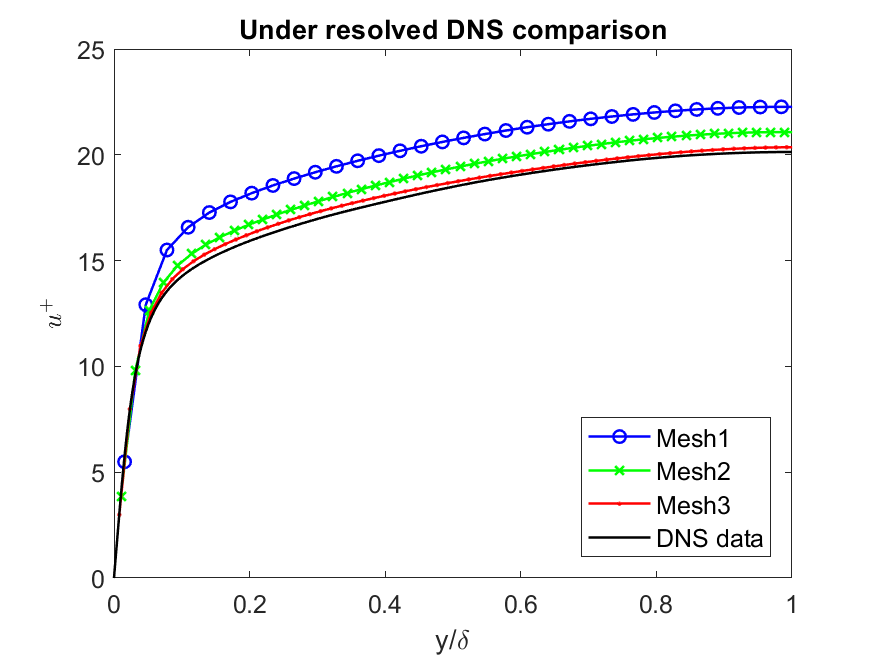
\includegraphics[width=0.95\textwidth]{06_Resultsanddiscussion/figur/UDNS_2016/Profile_global_coords.png}
%    \caption{Mean stream-wise velocity profile normalized by $u_\tau$, plotted in global coordinates}
%    \label{Mean velocity global}
%\end{figure}
%
%\begin{figure}[t]
%    \centering
%    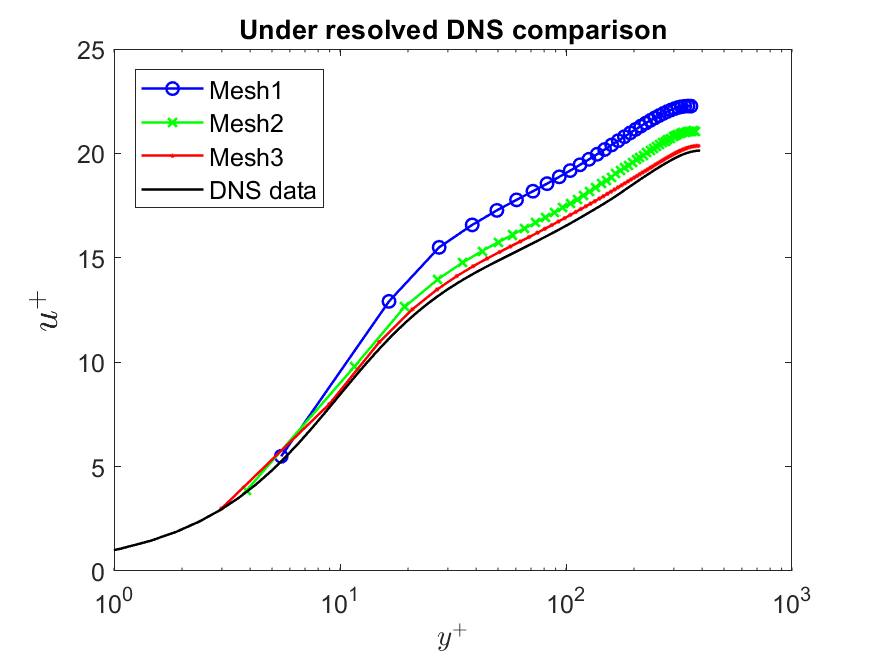
\includegraphics[width=0.95\textwidth]{06_Resultsanddiscussion/figur/UDNS_2016/Profile_wall_coords_theo_comp.png}
%    \caption{Mean stream-wise  velocity profile normalized by $u_\tau$, plotted in wall coordinates (semi-log plot)}
%    \label{Mean velocity wall}
%\end{figure}

\subsubsection{Turbulence intensities} \label{Turbulence intensities UDNS}
Turbulence intensities is the term used for the root-mean-square (rms) profiles of the velocity fluctuations. The rms profiles shown in this section have been averaged in the following order: 
the time-averaged data set written out in every time-step is spatially averaged and these time and space averaged data sets are again time-averaged to have symmetric rms profiles. The Fig. \ref{Turbulence intensities} shows the rms velocity fluctuations plotted in the global coordinates. The rms profiles are symmetric about the half-channel height i.e. $y = \de$ and the symmetry of the profiles about $\de$ indicates the adequacy of the sampling taken for average ~\cite{kim:moin:moser:87}. Turbulence intensities normalised by $u_\tau$ are compared with different mesh resolutions and the DNS data\footnote{the DNS data for the velocity fluctuation profiles have been provided as variances ($\overline{{\up}^2}$) and not the rms ($\sqrt{\overline{{\up}^2}}$)values}. 
%
\begin{figure}[h!]
    \centering
    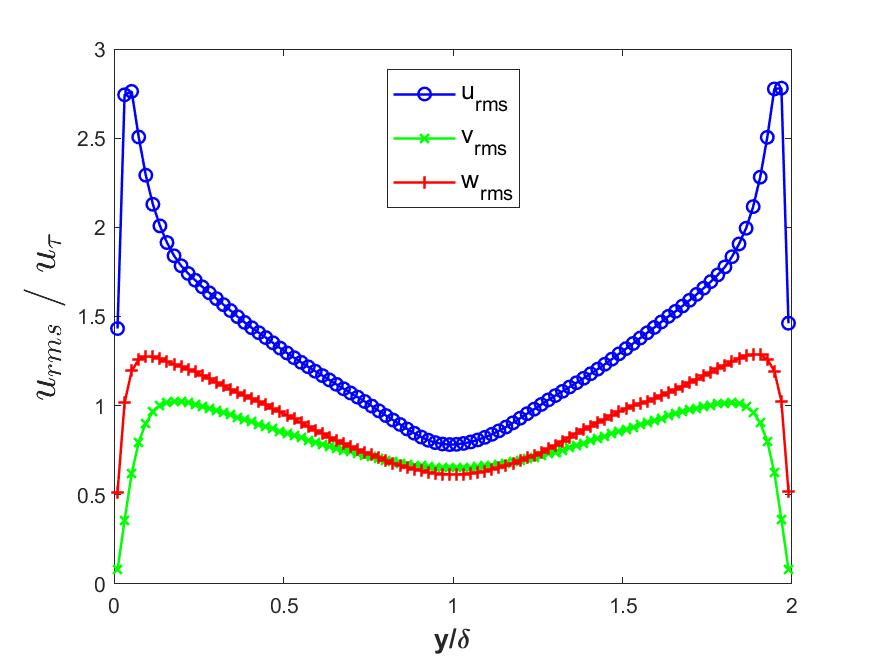
\includegraphics[width=0.6\textwidth]{06_Resultsanddiscussion/figur/UDNS_2016/Turbulence ontensities_Mesh2.jpg}
    \caption{Root-mean-square velocity fluctuations normalized by $u_\tau$ in global coordinates}
    \label{Turbulence intensities}
\end{figure}
%

Fig.(\ref{urms udns})-(\ref{wrms udns}) shows the comparison of the components of the rms profiles of the streamwise, wall-normal and spanwise velocity fluctuations, respectively, with the different mesh resolutions and the DNS data in wall coordinates. The profiles do not start from zero value, as only the fluid nodes are plotted. The general observation from all three velocity fluctuation profiles is that they converge to the DNS data with the increase in the mesh resolution. 

Mesh 2 and Mesh 3 accurately estimates the location of the peak values for all three velocity component profiles, respectively, compared to the DNS data. Mesh 3 for all the velocity component profiles predict the peak value fairly close to that of the DNS data. All three velocity component profiles for Mesh 3 are in fairly good agreement with the DNS data. 

The rms value of the streamwise profile increases from zero at the wall to some peak value in either buffer layer, $5<y^+< 30$, or in the log-law layer, $y^+ > 30\  till\  y/\de <0.3$ and then drops gradually towards the centre of the channel. The velocity profile for the wall-normal component develops slowly in comparison to the streamwise and the spanwise component profiles. The approximate location of the peak value for streamwise profile (DNS) is at $y^+ = 14$ \cite{kim:moin:moser:87} i.e. buffer layer. The location of peak value for the spanwise component (DNS) is at $y^+ = 40$ i.e. log-law region and the location for the wall-normal component (DNS)is at $y^+ = 70$ also in the log-law region, but towards the end of it. The resulting profiles of Mesh 3 for all components approximately shows the same locations for the peak values as that of the corresponding DNS data.
%%
%\begin{table}[h!]
%\begin{center}
%\begin{tabular}{ p{1cm}|p{1.5cm}p{1.5cm}p{1.5cm}p{1.5cm}  } 
%\hline
% & Mesh1 & Mesh2 & Mesh3 & DNS \\
%  \hline
%  \multirow{1}{6em}{$y^+$} & 17 & 15 & 14.93 & 14\\
%  \hline
%\end{tabular}
%\end{center}
%\caption{Peak values of the rms profiles of stream-wise velocity fluctuations}
%\label{Peak values}
%\end{table}
%%
%
\begin{figure}[h]
%\centering
\begin{minipage}[b]{0.5\textwidth}
\subfigure[global coordinates]{
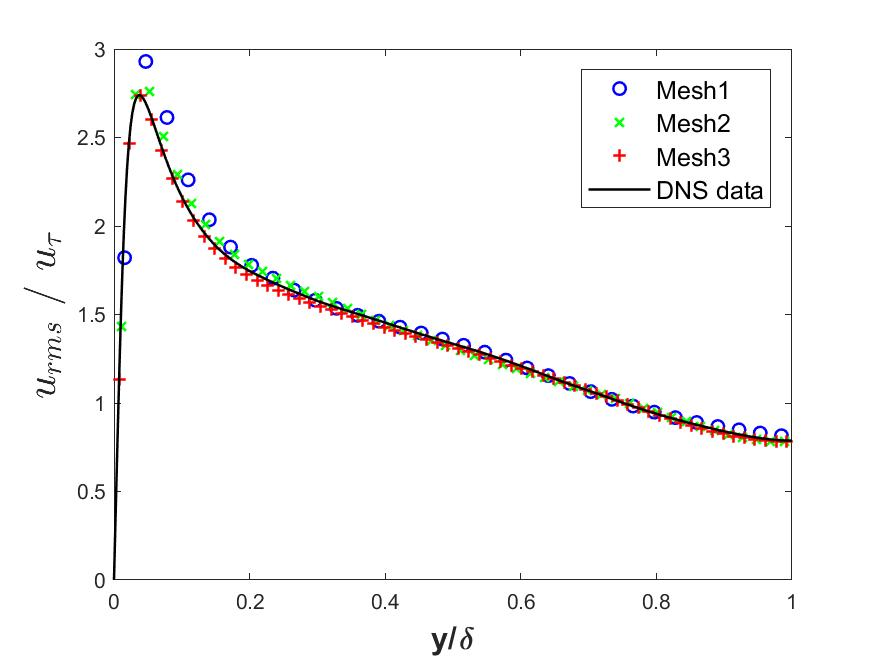
\includegraphics[width=6.7cm]{06_Resultsanddiscussion/figur/UDNS_2016/urms_global_coords.jpg}}
\end{minipage}
%
\begin{minipage}[b]{0.5\textwidth}
\subfigure[wall coordinates]{
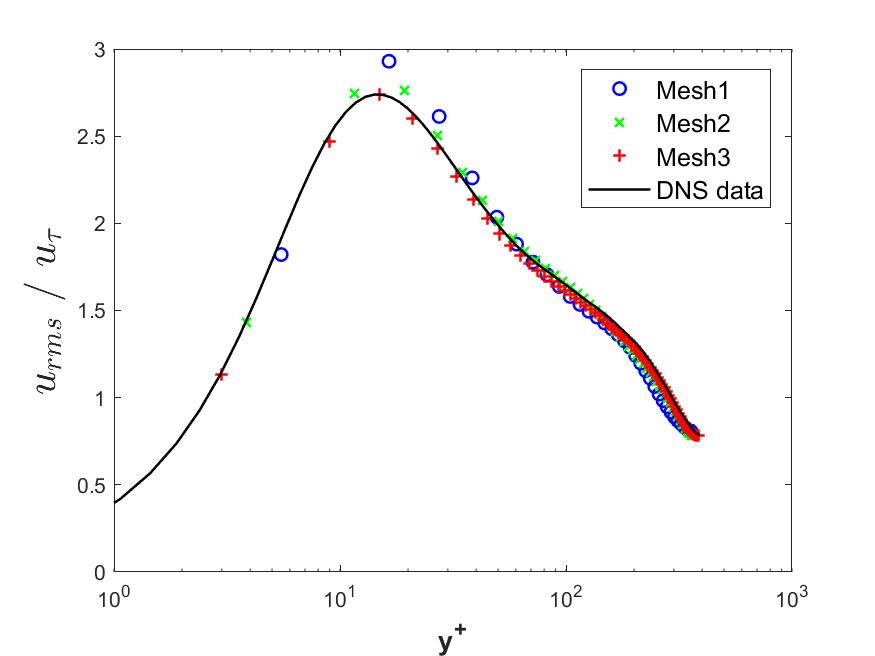
\includegraphics[width=6.7cm]{06_Resultsanddiscussion/figur/UDNS_2016/urms_wall_coords.jpg}}
\end{minipage}
\caption{Rms profiles for the streamwise velocity fluctuation normalised by $u_\tau$}
\label{urms udns}
\end{figure}

%% vrms %%
\begin{figure}[h]
\begin{minipage}[b]{0.5\textwidth}
\subfigure[global coordinates]{
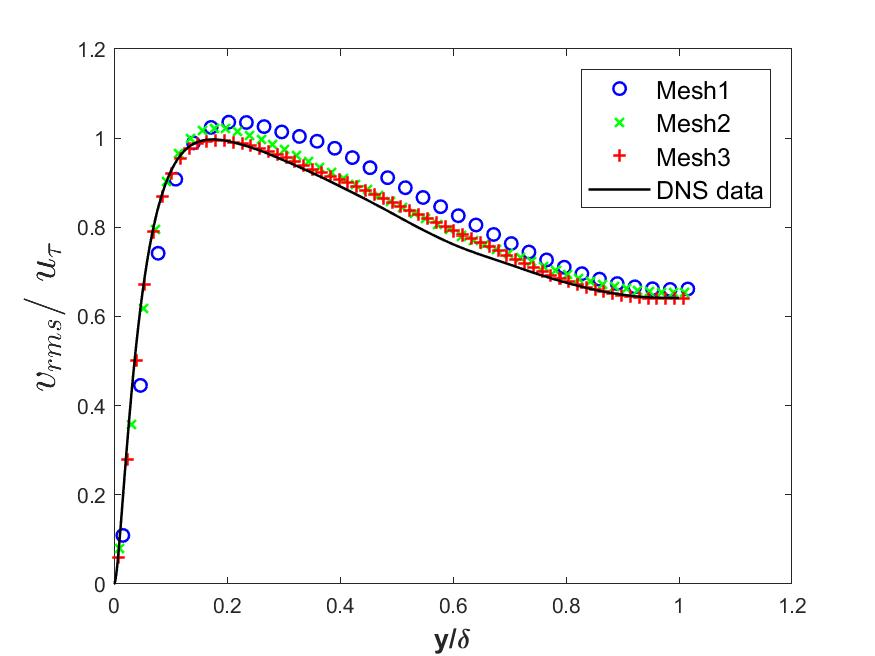
\includegraphics[width=6.7cm]{06_Resultsanddiscussion/figur/UDNS_2016/vrms_global_coords.jpg}}
\end{minipage}
%
\begin{minipage}[b]{0.5\textwidth}
\subfigure[wall coordinates]{
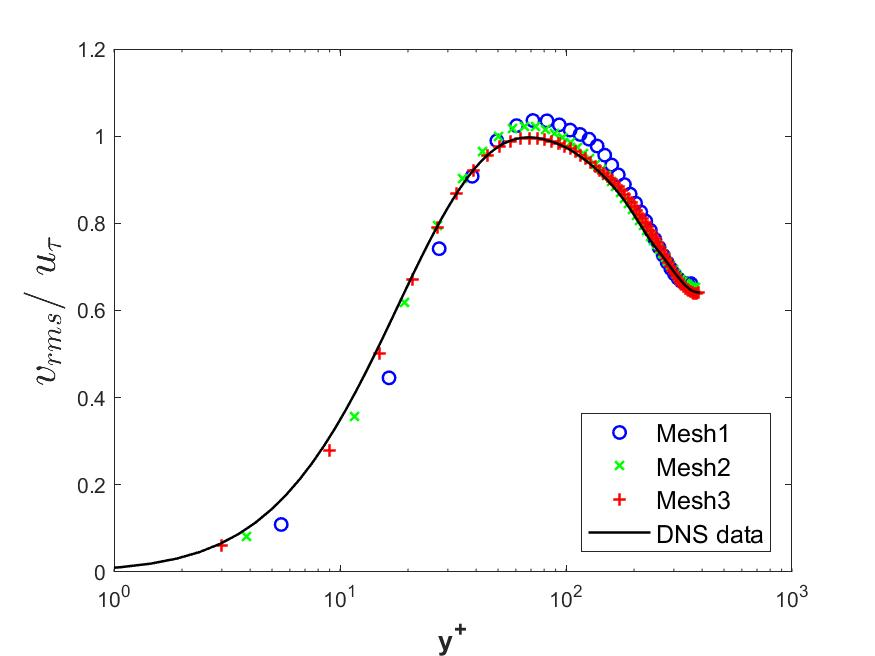
\includegraphics[width=6.7cm]{06_Resultsanddiscussion/figur/UDNS_2016/vrms_wall_coords.jpg}}
\end{minipage}
\caption{Rms profiles for the wall-normal velocity fluctuation normalised by $u_\tau$}
\label{vrms udns}
\end{figure}

%% wrms %%
\begin{figure}[h]
\begin{minipage}[b]{0.5\textwidth}
\subfigure[global coordinates]{
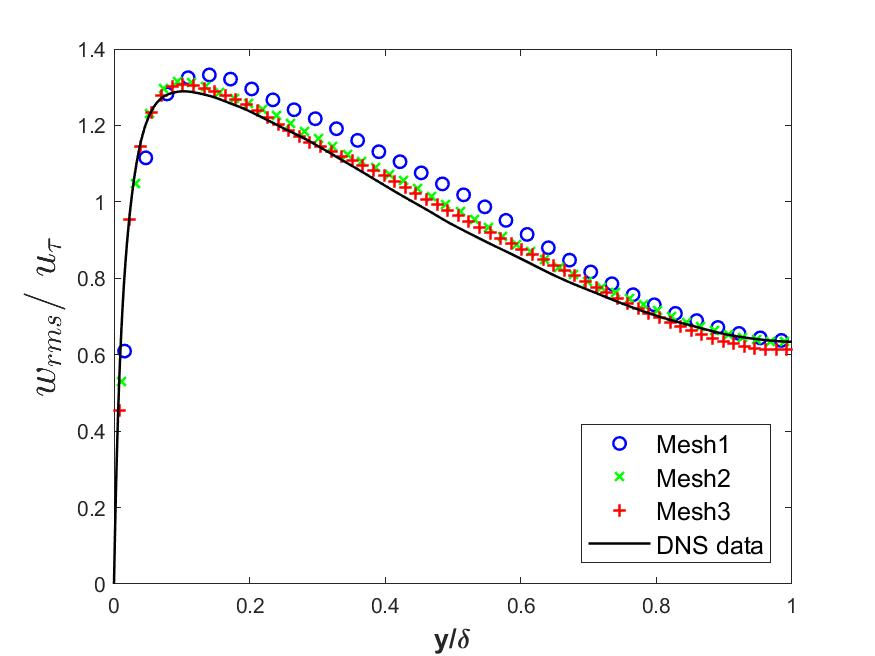
\includegraphics[width=6.7cm]{06_Resultsanddiscussion/figur/UDNS_2016/wrms_global_coords.jpg}}
\end{minipage}
%
\begin{minipage}[b]{0.5\textwidth}
\subfigure[wall coordinates]{
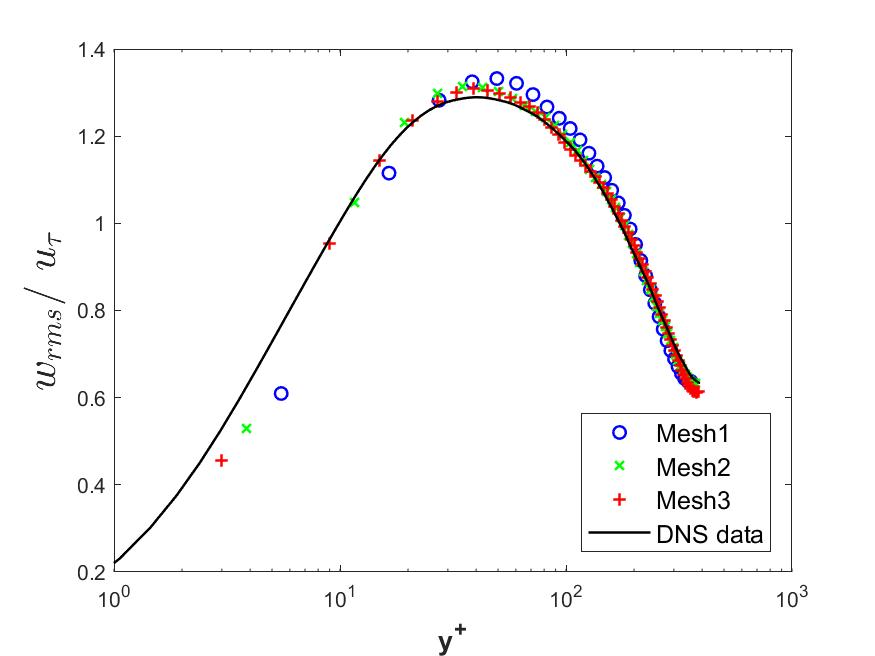
\includegraphics[width=6.7cm]{06_Resultsanddiscussion/figur/UDNS_2016/wrms_wall_coords.jpg}}
\end{minipage}
\caption{Rms profiles for the spanwise velocity fluctuation normalised by $u_\tau$}
\label{wrms udns}
\end{figure}

%\begin{figure}[h!]
%    \centering
%    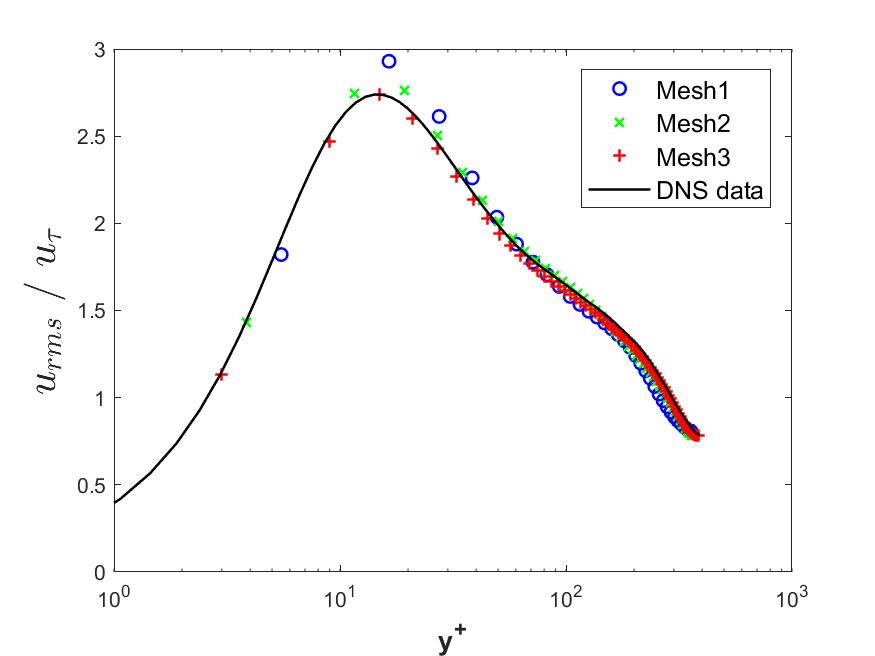
\includegraphics[width=0.6\textwidth]{06_Resultsanddiscussion/figur/UDNS_2016/urms_wall_coords.jpg}
%    \caption{$u_{rms}$ normalized by $u_\tau$ in wall coordinates}
%    \label{urms wall}
%\end{figure}

%\begin{figure}[h!]
%    \centering
%    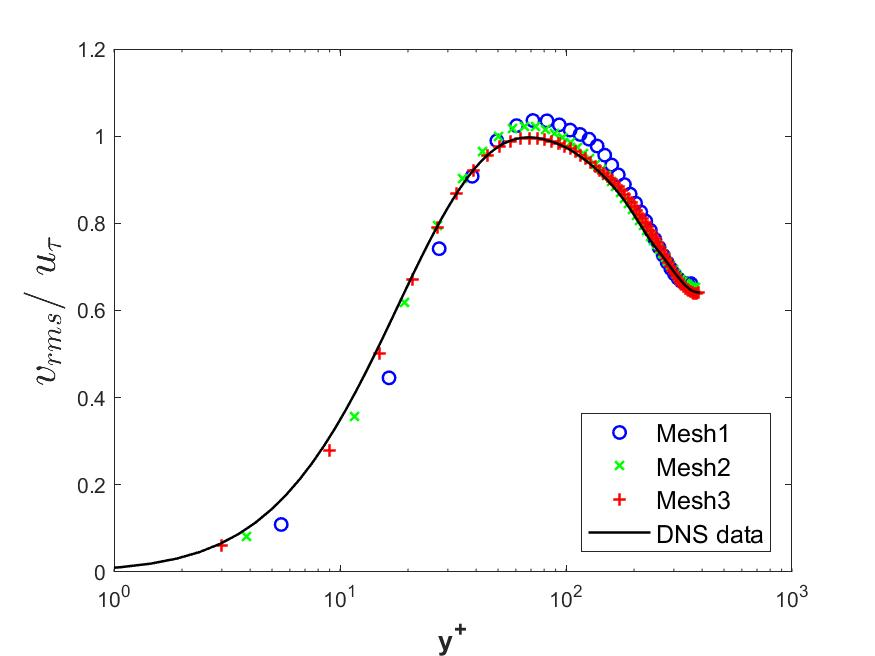
\includegraphics[width=0.6\textwidth]{06_Resultsanddiscussion/figur/UDNS_2016/vrms_wall_coords.jpg}
%    \caption{$v_{rms}$ normalized by $u_\tau$ in wall coordinates}
%    \label{vrms wall}
%\end{figure}

%\begin{figure}[h!]
%    \centering
%    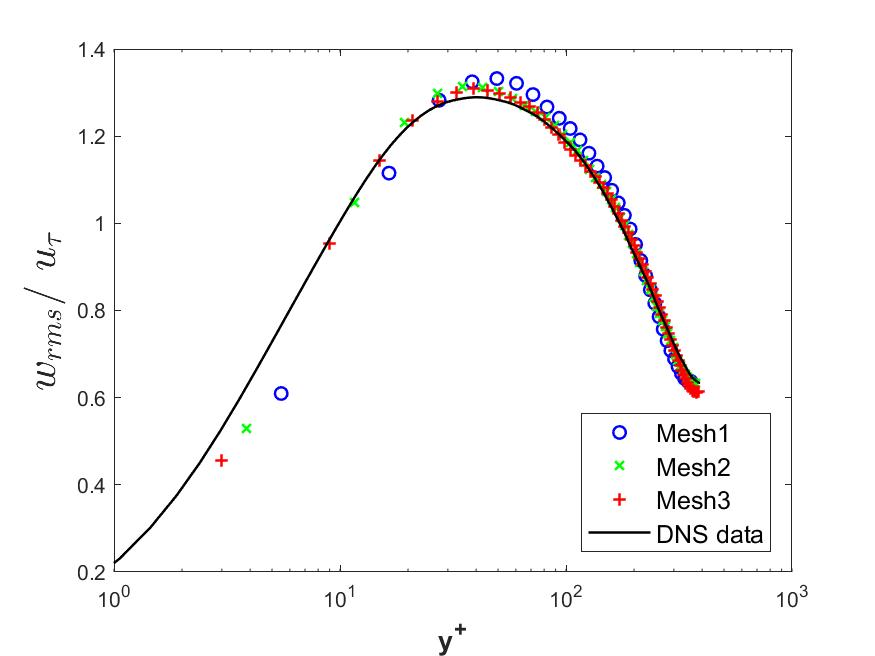
\includegraphics[width=0.6\textwidth]{06_Resultsanddiscussion/figur/UDNS_2016/wrms_wall_coords.jpg}
%    \caption{$w_{rms}$ normalized by $u_\tau$ in wall coordinates}
%    \label{wrms wall}
%\end{figure}

\subsubsection{Turbulent shear stress}
Turbulent shear stress is also referred to as the co-variance of the Reynolds stress tensor i.e. $-\overline{\up\vp}$. This component is responsible for the turbulent diffusion of the momentum. It is also sometimes referred to as the resolved shear stress. 

Fig. (\ref{uvrms udns}) shows the turbulent shear stress profile normalised with the $u_\tau^2$ plotted in wall coordinates and compared against the DNS data and with the mesh resolutions. As seen from the Fig. (\ref{uvrms udns}) the increase in the mesh resolution results in the better agreement to the DNS data. Mesh 3 here shows a very good agreement to the DNS data and also it predicts the location of the peak value, $y^+ = 35$ fairly well.

%% uv_rms %%
\begin{figure}[h]
\begin{minipage}[b]{0.5\textwidth}
\subfigure[global coordinates]{
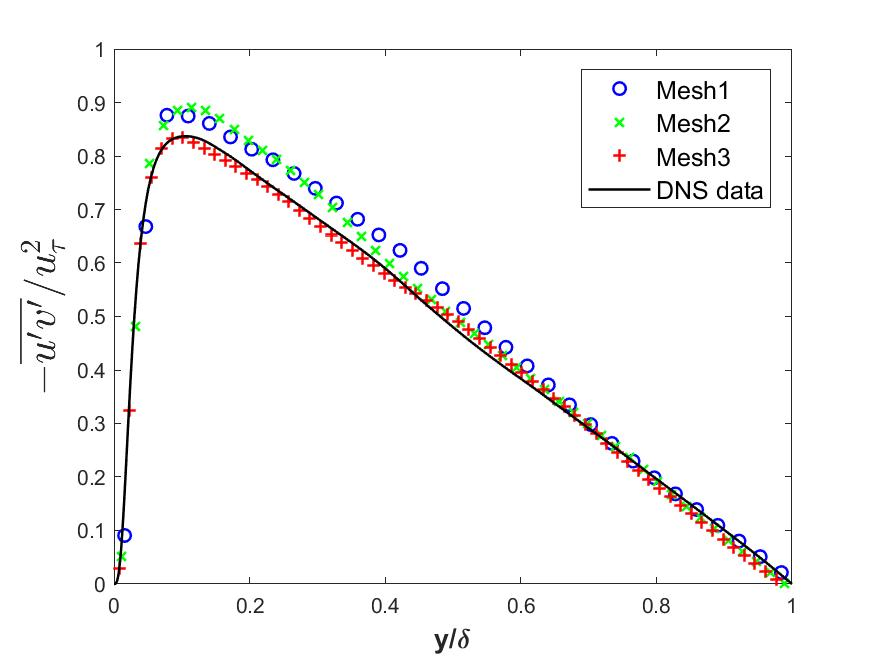
\includegraphics[width=6.7cm]{06_Resultsanddiscussion/figur/UDNS_2016/uv_rms_global_coords.jpg}}
\end{minipage}
%
\begin{minipage}[b]{0.5\textwidth}
\subfigure[wall coordinates]{
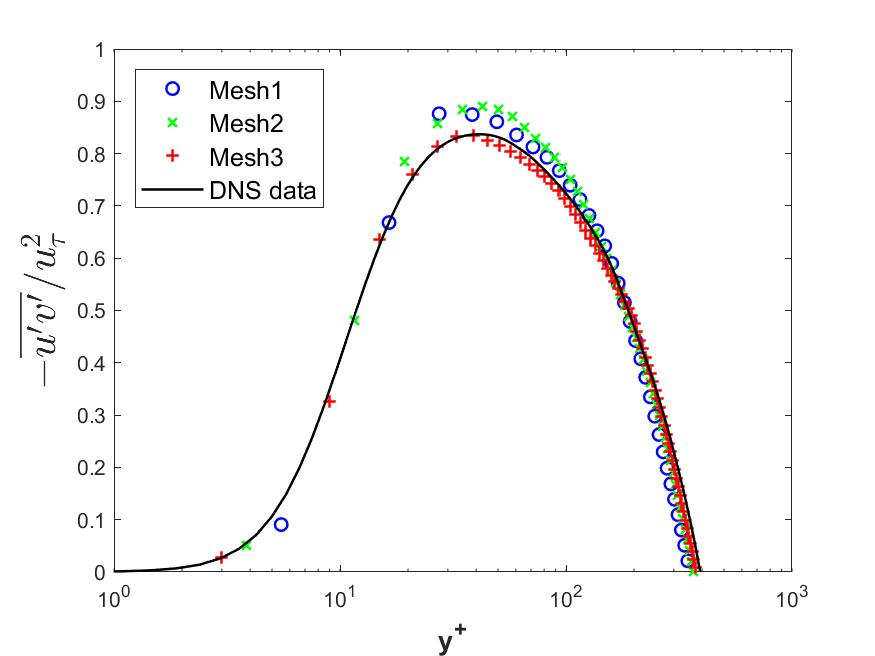
\includegraphics[width=6.7cm]{06_Resultsanddiscussion/figur/UDNS_2016/uv_rms_wall_coords.jpg}}
\end{minipage}
\caption{Turbulent shear stress normalised by $u_\tau^2$}
\label{uvrms udns}
\end{figure}

%\begin{figure}[h!]
%    \centering
%    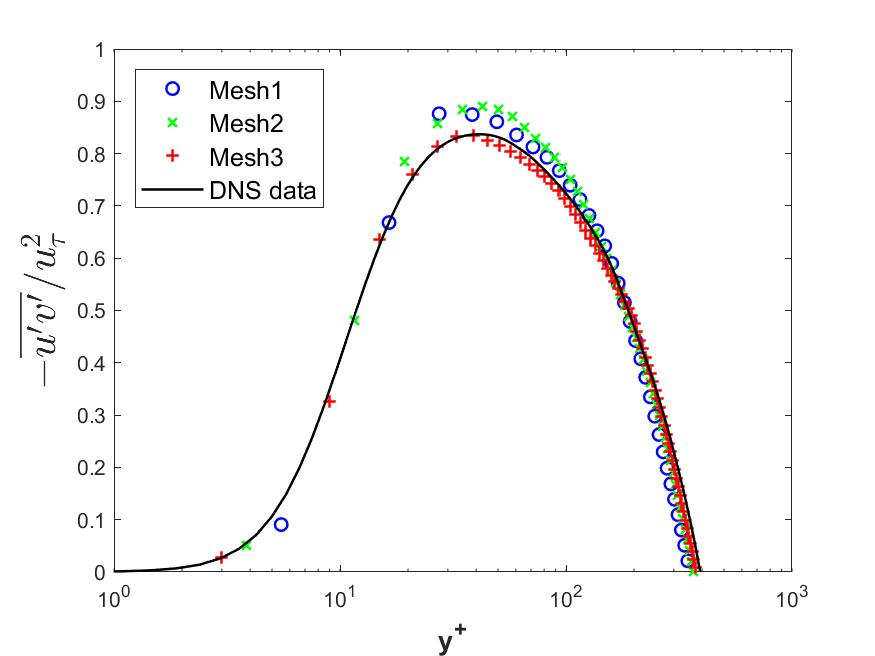
\includegraphics[width=0.6\textwidth]{06_Resultsanddiscussion/figur/UDNS_2016/uv_rms_wall_coords.jpg}
%    \caption{$uv_{rms}$ normalized by $u_\tau$ in wall coordinates}
%    \label{uvrms wall}
%\end{figure}
\subsection{WALE model results}
In this section the results obtained from the combination of the LB flow solver with the WALE model (LES) performed on the relatively coarser mesh, in comparison to the resolution of the DNS data, will be presented. The main purpose is to access the accuracy with which the aforementioned combination reproduces the mean flow profiles and other turbulence statistics when compared to the DNS data. The computed physical quantities have been listed in the table \ref{Global quantities WALE} for all mesh resolutions. The same trend is seen for the physical quantities as mentioned in the section \ref{UDNS profiles}. The physical quantities approach closer to the respective target values with the increase in the mesh resolution. 
%
\begin{table}[h!]
\begin{center}
\begin{tabular}{ p{3cm}|p{1.5cm}p{1.5cm}p{1.5cm}p{1.5cm}  } 
\hline
Physical quantity & Mesh1 & Mesh2 & Mesh3 & Target \\
  \hline
  \multirow{1}{6em}{$u_\tau,\ m/s$}  & 0.0069 & 0.0073 & 0.0075 & 0.0079\\
  \hline
  \multirow{1}{6em}{$Re_\tau$} & 347 & 367 & 377 & 395\\
  \hline
  \multirow{1}{6em}{$U_c,\ m/s$} & 0.1562 & 0.1557 & 0.1547 & 0.1591\\
  \hline
\end{tabular}
\end{center}
\caption{Comparison of the computed physical quantities using WALE model}
\label{Global quantities WALE}
\end{table}
%
\subsubsection{Mean velocity profiles}
The mean velocity profiles, normalised with the $u_\tau$, presented here are averaged in time and space. Fig. (\ref{Mean profiles WALE}(a-b)) shows the mean velocity profiles plotted in the global and local coordinates. It is clear from the both the figures that with increase in the mesh resolution the velocity profiles approach closer to the DNS data. All profiles over-predict the DNS data, but the velocity profile for the mesh 3 is relatively in good agreement with the DNS data. The reason for the over-prediction is similar to that explained in section \ref{Mean velocity UDNS}.
%%% Mean veloity profiles %%%
\begin{figure}[h!]
%\centering
\begin{minipage}[b]{0.5\textwidth}
\subfigure[global coordinates]{
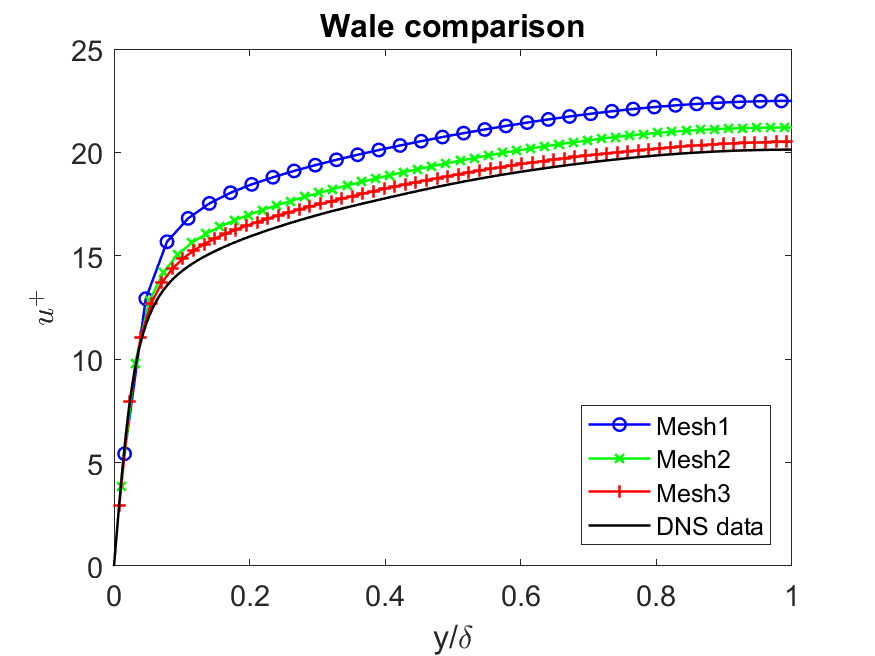
\includegraphics[width=6.7cm]{06_Resultsanddiscussion/figur/WALE/Profile_global_coords.png}}
\end{minipage}
%
\begin{minipage}[b]{0.5\textwidth}
\subfigure[wall coordinates]{
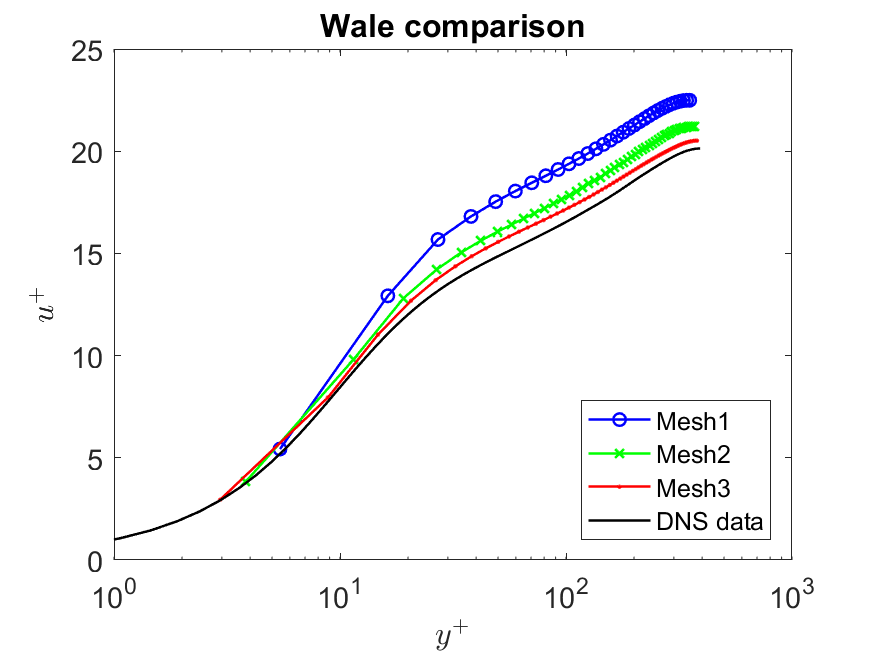
\includegraphics[width=6.7cm]{06_Resultsanddiscussion/figur/WALE/Profile_wall_coords_theo_comp.png}}
\end{minipage}
\caption{Mean velocity profile normalised with $u_\tau$}
\label{Mean profiles WALE}
\end{figure}
%%% End mean velociy profiles %%%%
\subsubsection{Turbulence intensities}
The rms profiles presented here are averaged in the same fashion as that of the section \ref{Turbulence intensities UDNS}. To show the adequacy of sampling taken for averaging the symmetric rms profiles, about the half-channel height $y  = \de$, of all three velocity fluctuations is shown in Fig. (\ref{Turbulence intensities WALE}). The comments made in the section \ref{Turbulence intensities UDNS} for the velocity profiles are also applicable here.
The rms velocity profiles for all three components show a good agreement towards the DNS data as the mesh resolution increases.
%
\begin{figure}[h!]
    \centering
    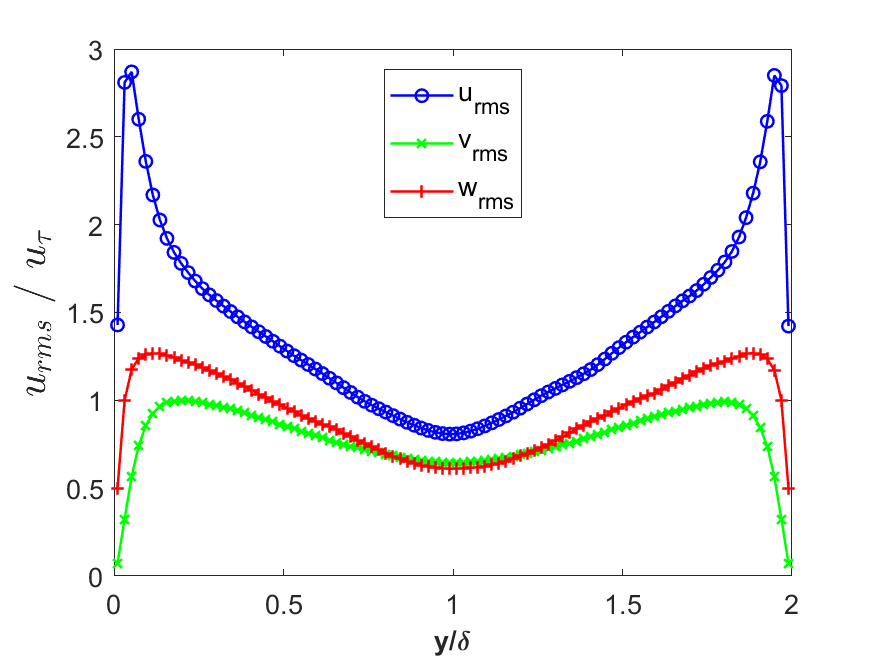
\includegraphics[width=0.6\textwidth]{06_Resultsanddiscussion/figur/WALE/Turbulence intensities_Mesh2.png}
    \caption{Root-mean-square velocity fluctuations normalized by $u_\tau$ in global coordinates}
    \label{Turbulence intensities WALE}
\end{figure}
%

From Fig. (\ref{urms wale}) it is clear that the location of the peak value is predicted nearly correctly by rms profile of mesh 3. Rms profiles of all meshes overpredict the reference(DNS data) peak value. Overall mesh 3 shows a better agreement to the DNS data, although with a slight overprediction of the peak value. 
%
\begin{figure}[h!]
%\centering
\begin{minipage}[b]{0.5\textwidth}
\subfigure[global coordinates]{
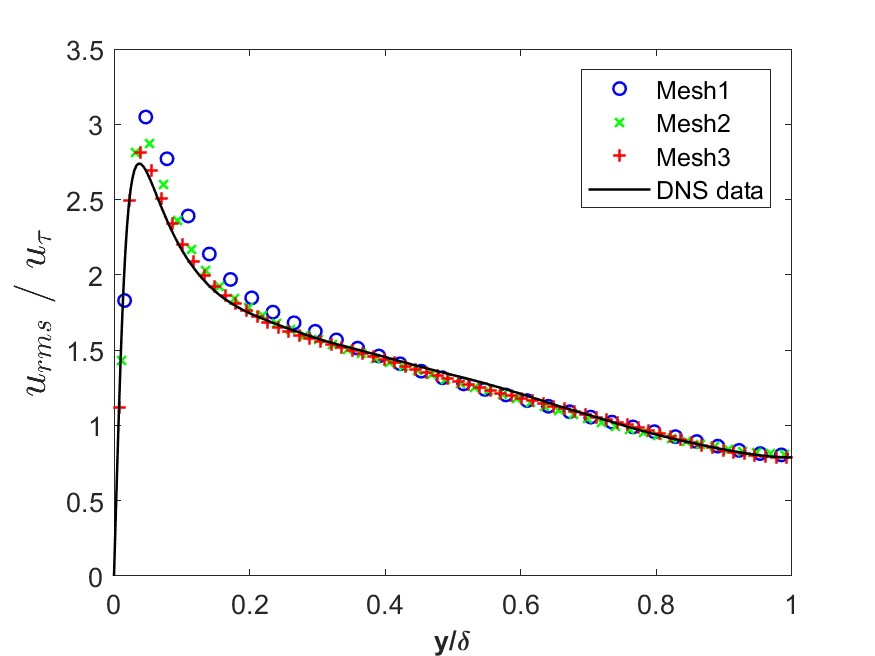
\includegraphics[width=6.7cm]{06_Resultsanddiscussion/figur/WALE/urms_global_coords.png}}
\end{minipage}
%
\begin{minipage}[b]{0.5\textwidth}
\subfigure[local coordinates]{
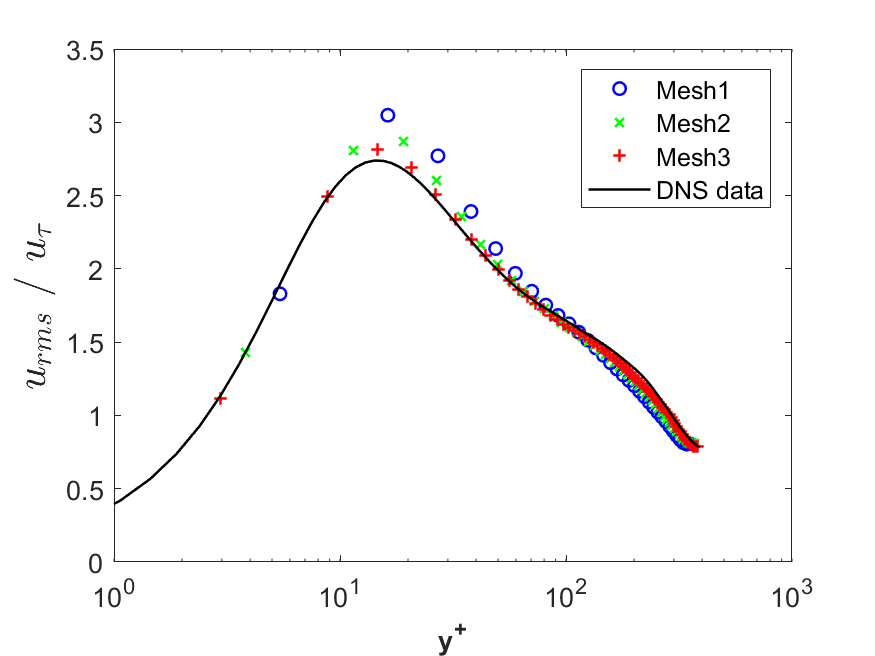
\includegraphics[width=6.7cm]{06_Resultsanddiscussion/figur/WALE/urms_wall_coords.png}}
\end{minipage}
\caption{Rms profiles for the streamwise velocity fluctuation normalised by $u_\tau$}
\label{urms wale}
\end{figure}
%% End %%

From Fig. (\ref{vrms wale}) it appears that profile for mesh 1 is shifted towards the right and so is the location of the peak value. With mesh refinement the profiles shift towards the left and the peak value is under-predicted by mesh 1 and mesh 3. Mesh 2 somehow overpredicts the peak value. All profiles underpredict in the viscous sublayer (mesh 2 and mesh 3) and the buffer layer. Resolution for mesh 3 approximates the DNS data quite well, although, with some underprediction in the log-law layer i.e. peak value.
%
\begin{figure}[h!]
%\centering
\begin{minipage}[b]{0.5\textwidth}
\subfigure[global coordinates]{
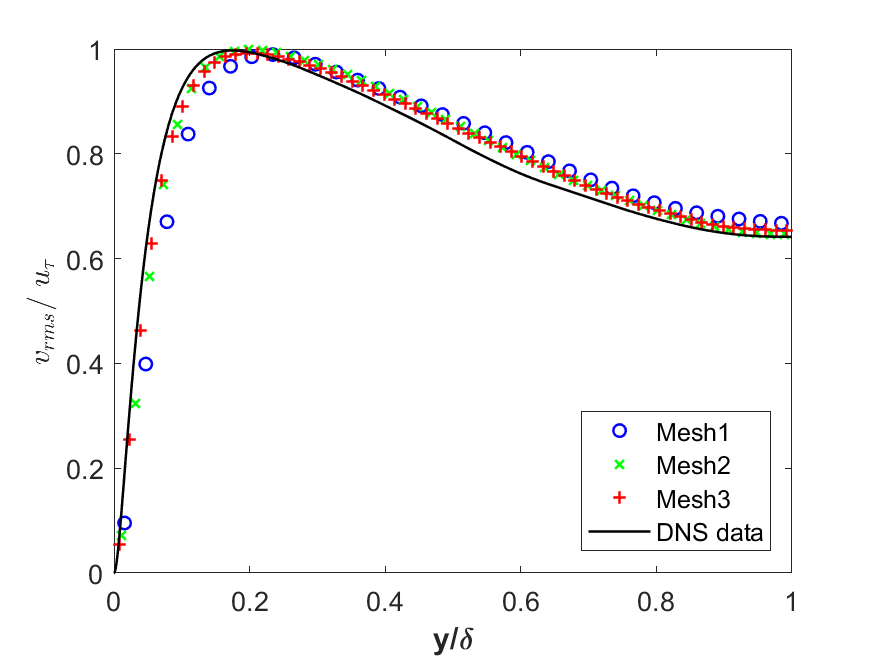
\includegraphics[width=6.7cm]{06_Resultsanddiscussion/figur/WALE/vrms_global_coords.png}}
\end{minipage}
%
\begin{minipage}[b]{0.5\textwidth}
\subfigure[local coordinates]{
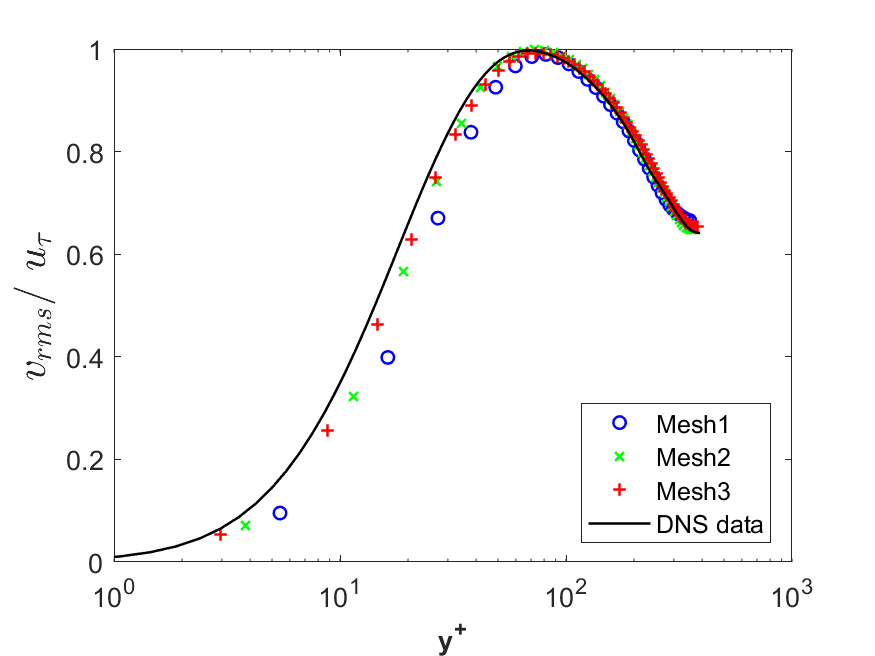
\includegraphics[width=6.7cm]{06_Resultsanddiscussion/figur/WALE/vrms_wall_coords.png}}
\end{minipage}
\caption{Rms profiles for the wall-normal velocity fluctuation normalised by $u_\tau$}
\label{vrms wale}
\end{figure}
%% End %%

Fig. (\ref{wrms wale}) shows that all the profiles overpredict the location of the peak values and also the peak values. Mesh 3 shows a better agreement with the DNS data, with some overprediction in the log-law layer.
%
\begin{figure}[h!]
%\centering
\begin{minipage}[b]{0.5\textwidth}
\subfigure[global coordinates]{
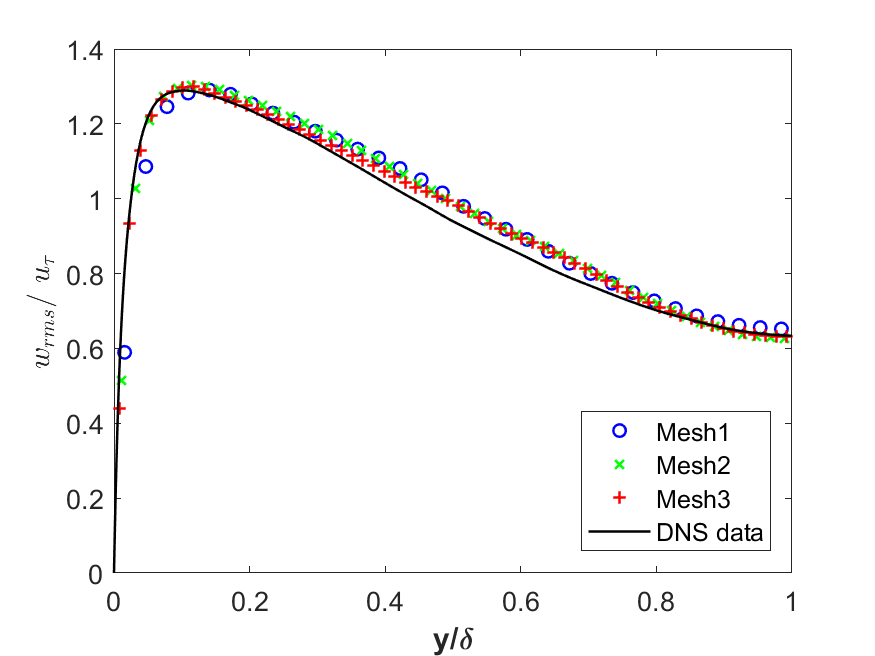
\includegraphics[width=6.7cm]{06_Resultsanddiscussion/figur/WALE/wrms_global_coords.png}}
\end{minipage}
%
\begin{minipage}[b]{0.5\textwidth}
\subfigure[local coordinates]{
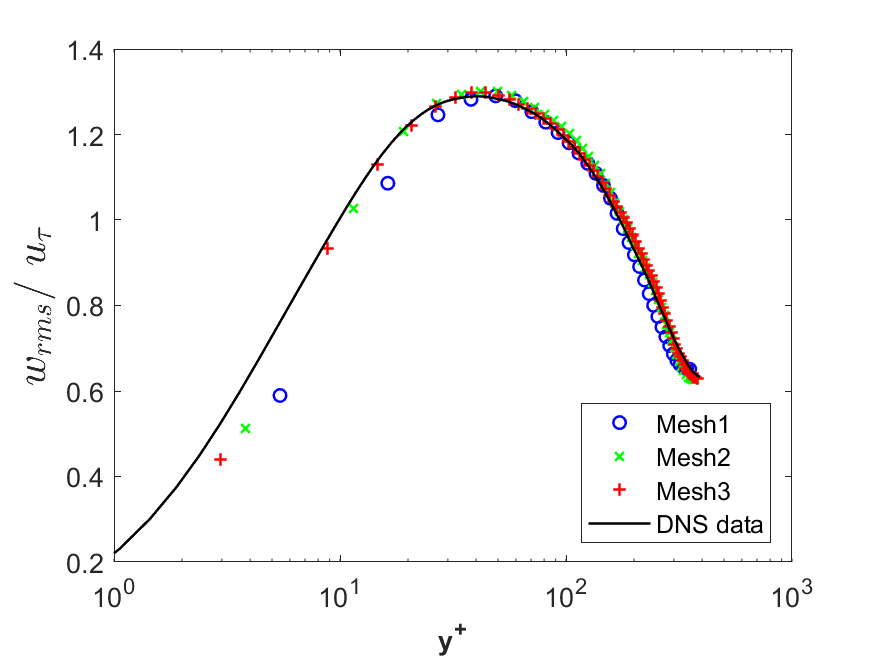
\includegraphics[width=6.7cm]{06_Resultsanddiscussion/figur/WALE/wrms_wall_coords.png}}
\end{minipage}
\caption{Rms profiles for the spanwise velocity fluctuation normalised by $u_\tau$}
\label{wrms wale}
\end{figure}
%% End %%
\subsubsection{Turbulent shear stress}
Fig. (\ref{uvrms wale}) shows the turbulent shear stress normalised by $u_\tau^2$ plotted in global and wall coordinates. Mesh 1 and mesh 2 overpredicts the DNS data in the log-law layer and eventually the peak value. Profile for mesh 3 completely collapses on to the DNS data.
%
\begin{figure}[h!]
%\centering
\begin{minipage}[b]{0.5\textwidth}
\subfigure[global coordinates]{
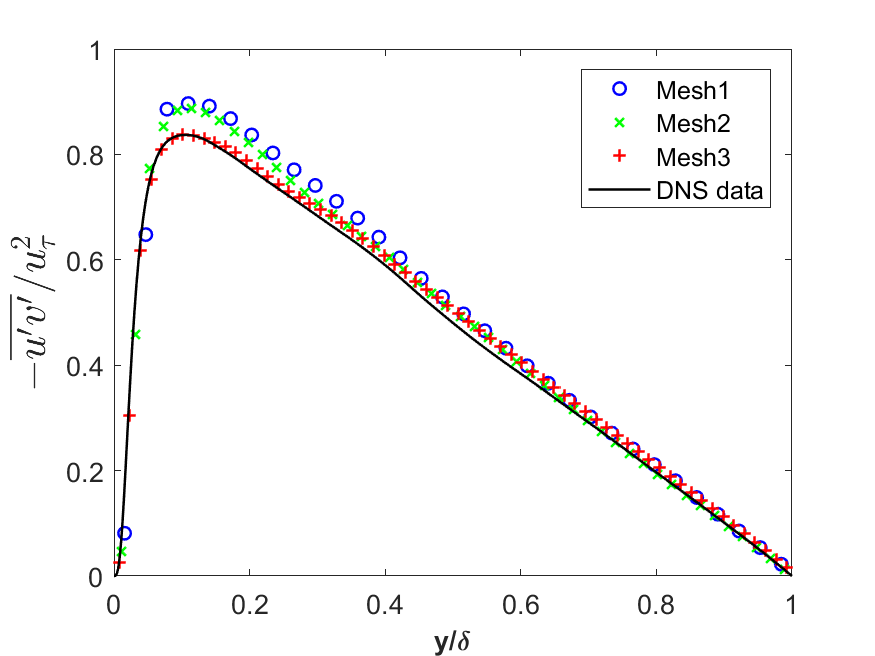
\includegraphics[width=6.7cm]{06_Resultsanddiscussion/figur/WALE/uv_rms_global_coords.png}}
\end{minipage}
%
\begin{minipage}[b]{0.5\textwidth}
\subfigure[local coordinates]{
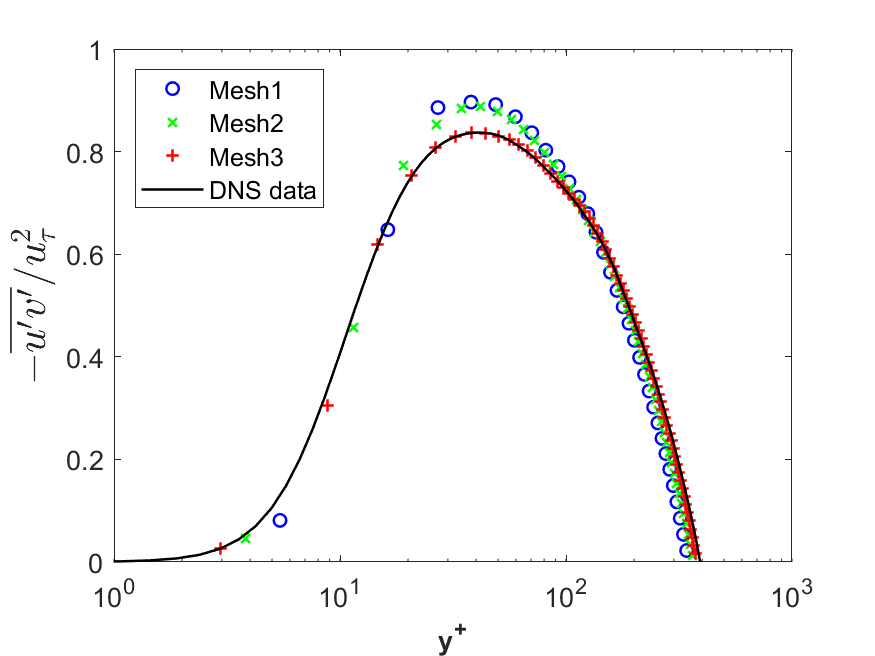
\includegraphics[width=6.7cm]{06_Resultsanddiscussion/figur/WALE/uv_rms_wall_coords.png}}
\end{minipage}
\caption{Turbulent shear stress profiles normalised by $u_\tau$}
\label{uvrms wale}
\end{figure}
%% End %%

\subsection{Comparison UDNS and WALE, $Re_\tau = 395$}

In this section a comparison will be made between the UDNS and WALE model results. The purpose of this comparison is to see how accurately does the combination of LB solver and WALE model predict the results in comparison to that of the UDNS results. Simultaneously they will also be compared with the DNS data. Only the comparison for the mesh 3 will be shown in here and the comparison for other resolution will be shown in the Appendix. From the table (\ref{Global quantities}) and (\ref{Global quantities WALE}) it can be seen that $u_\tau$ and the resulting $Re_\tau$ for the WALE model are smaller in comparison with that of the UDNS.

\subsubsection{Mean velocity profile}
Fig. (\ref{mean profiles udns vs wale global coords}) and Fig. (\ref{mean profiles udns vs wale wall coords}) show the comparison of the mean velocity profiles, normalised by $u_\tau$, with the results of UDNS, WALE and the DNS data in global and wall coordinates. Both the profiles overpredict the DNS data. The profile of WALE shows a slight more overprediction in comparison to the UDNS profile.
%
\begin{figure}[h!]
\begin{minipage}[b]{0.5\textwidth}
\subfigure[global coordinates]{
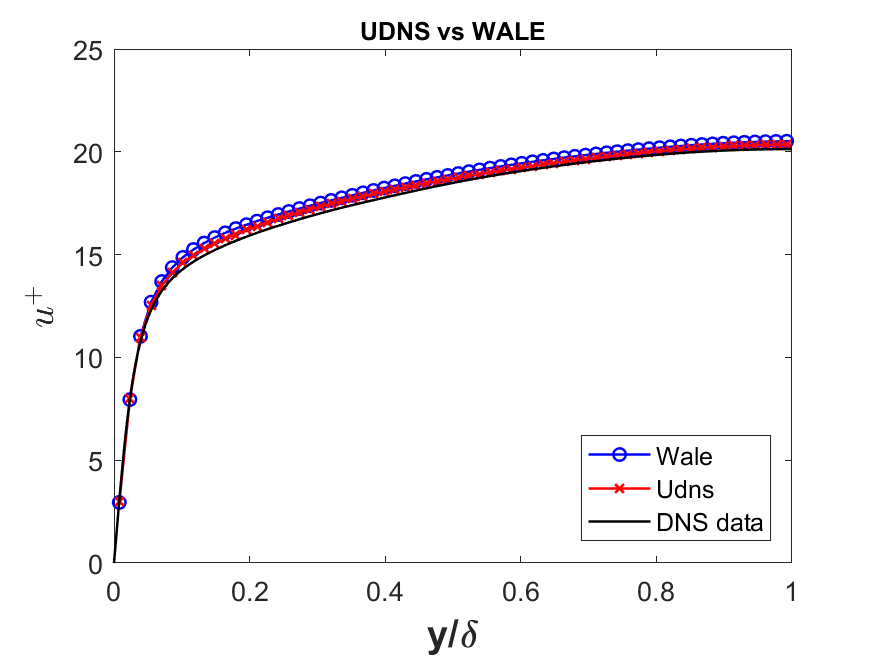
\includegraphics[width=6.7cm]{06_Resultsanddiscussion/figur/UDNSvsWale/Profile_global_coords.png}}
\end{minipage}
%
\begin{minipage}[b]{0.5\textwidth}
\subfigure[zoom in fig. (a)]{
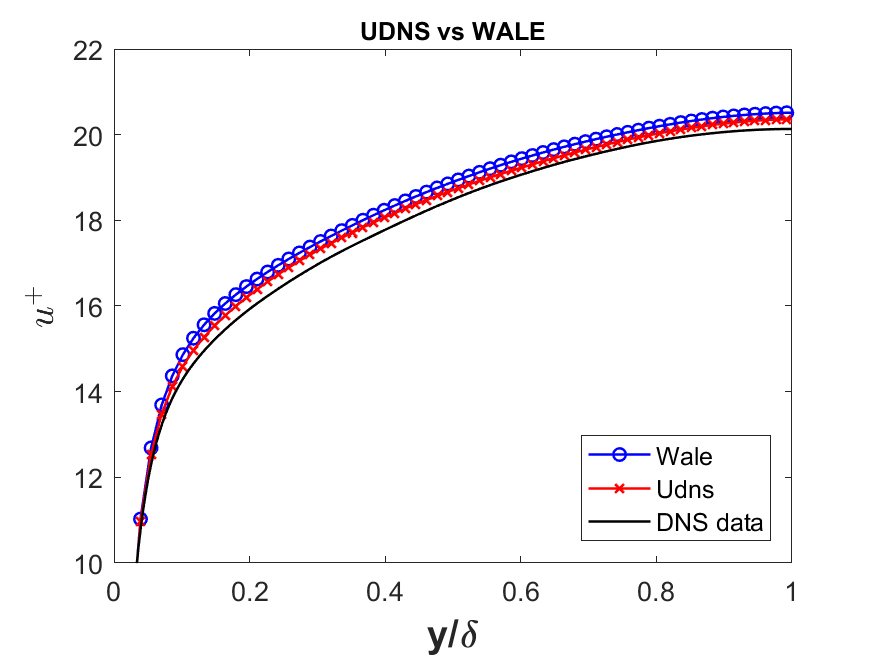
\includegraphics[width=6.7cm]{06_Resultsanddiscussion/figur/UDNSvsWale/Profile_global_coords_zoom.png}}
\end{minipage}
\caption{Mean velocity profiles normalised by $u_\tau$}
\label{mean profiles udns vs wale global coords}
\end{figure} 
%

%
\begin{figure}[h!]
\begin{minipage}[b]{0.5\textwidth}
\subfigure[wall coordinates]{
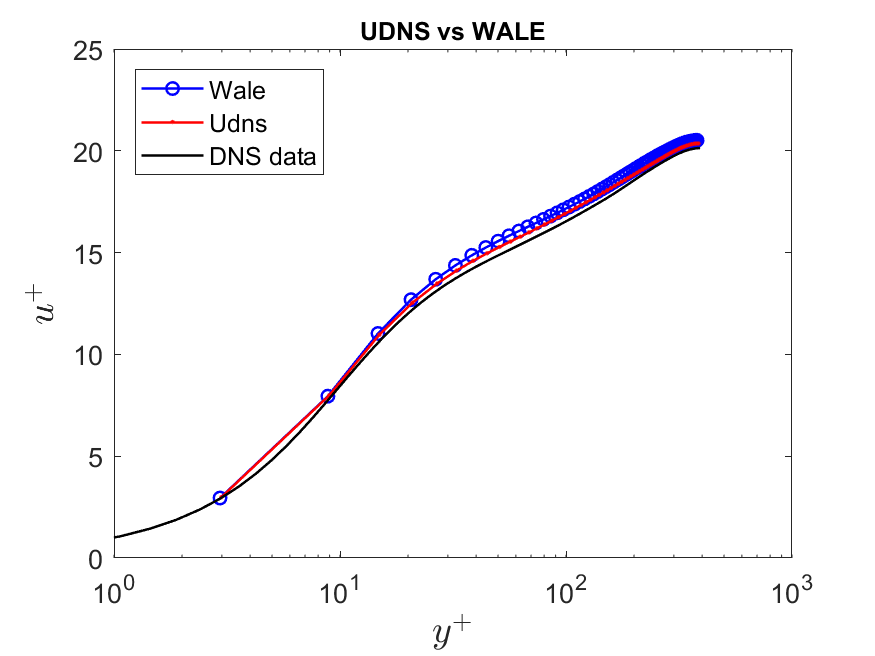
\includegraphics[width=6.7cm]{06_Resultsanddiscussion/figur/UDNSvsWale/Profile_wall_coords_theo_comp.png}}
\end{minipage}
%
\begin{minipage}[b]{0.5\textwidth}
\subfigure[zoom in fig. (a)]{
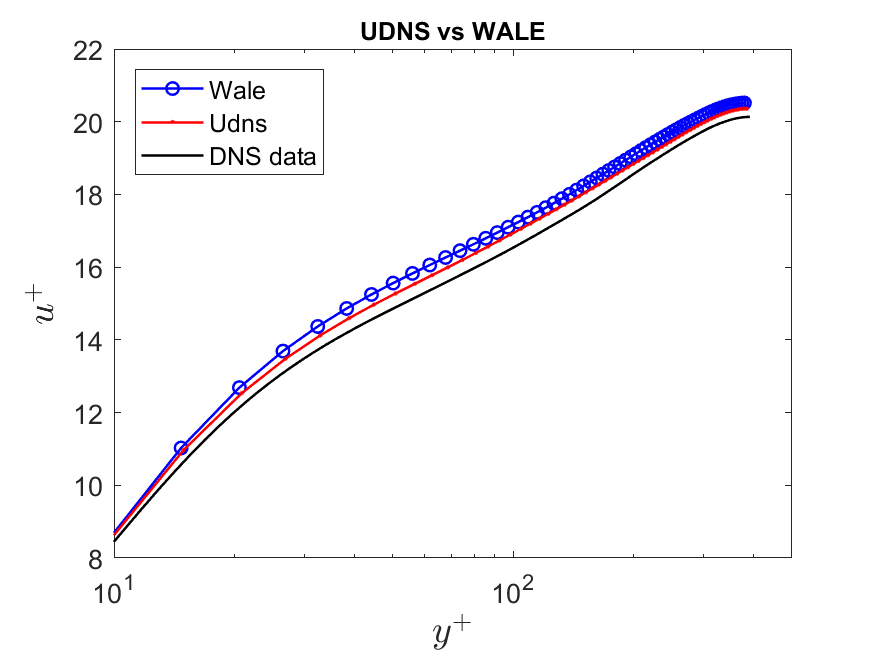
\includegraphics[width=6.7cm]{06_Resultsanddiscussion/figur/UDNSvsWale/Profile_wall_coords_theo_comp_zoom.png}}
\end{minipage}
\caption{Mean velocity profiles normalised by $u_\tau$}
\label{mean profiles udns vs wale wall coords}
\end{figure} 
%
The general explanation for the overprediction is the resulting $u_\tau$ being smaller, for WALE \& UDNS,  in comparison to the DNS data. The same applies to the overpredicting profile of the WALE in comparison to the UDNS profile. Ideally, both profiles, WALE \& UDNS, should underpredict the reference profile as we perform the simulations using under resolved mesh. This behaviour can be seen when we plot just the mean velocity and not the normalised mean velocity, $u^+$. Fig. \ref{mean profiles}(a) shows the mean velocity profile in the global coordinates and the Fig. \ref{mean profiles}(b) shows the zoomed in view of the mean velocity profile. It can be clearly seen that both UDNS \& WALE model underpredicts the reference mean centreline velocity, $U_c$. Profile for the WALE has the smallest centreline velocity. Thus, the comparison between the profiles of UDNS and WALE with each other as well as with the DNS data does not show any drastic difference. A marginal difference is seen between the profiles of the UDNS and WALE.

%
\begin{figure}[h!]
\begin{minipage}[b]{0.5\textwidth}
\subfigure[global coordinates]{
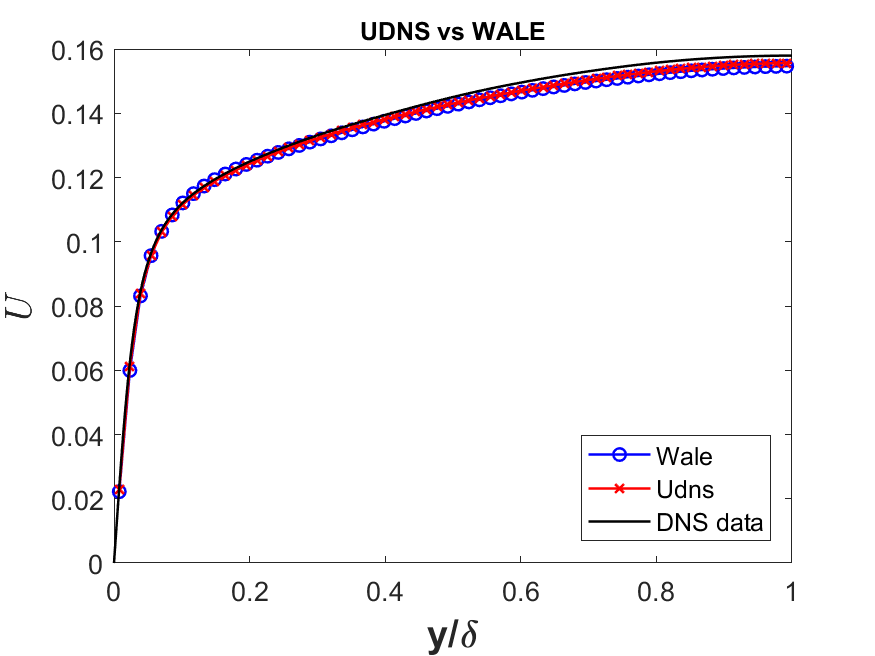
\includegraphics[width=6.7cm]{06_Resultsanddiscussion/figur/UDNSvsWale/Profile_global_coords_U.png}}
\end{minipage}
%
\begin{minipage}[b]{0.5\textwidth}
\subfigure[zoom in fig. (a)]{
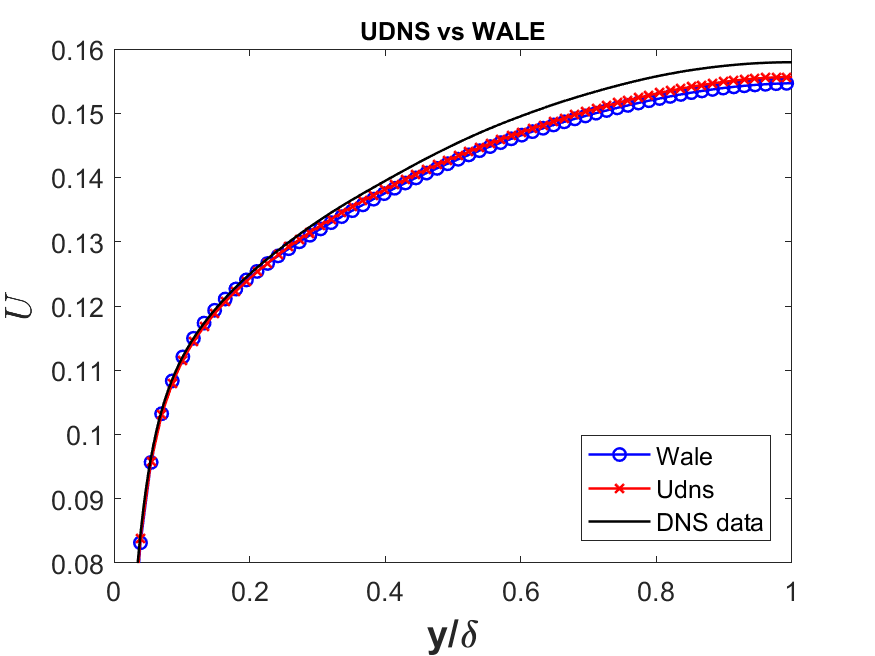
\includegraphics[width=6.7cm]{06_Resultsanddiscussion/figur/UDNSvsWale/Profile_global_coords_U_zoom.png}}
\end{minipage}
\caption{Mean velocity profiles}
\label{mean profiles}
\end{figure} 
%

\subsubsection{Turbulence intensities}
Fig. (\ref{urms udns vs wale}) shows the comparison of the $u_{rms}$ profiles of UDNS and WALE with each other  and also with the profile of the DNS data. Profiles of UDNS and WALE show a good agreement with the DNS data with the profile of WALE slightly overpredicting the peak value in the buffer layer. Apart from the slight overprediction in the buffer layer, the profiles for UDNS and WALE are also in good agreement with each other.
%
\begin{figure}[h!]
\begin{minipage}[b]{0.5\textwidth}
\subfigure[global coordinates]{
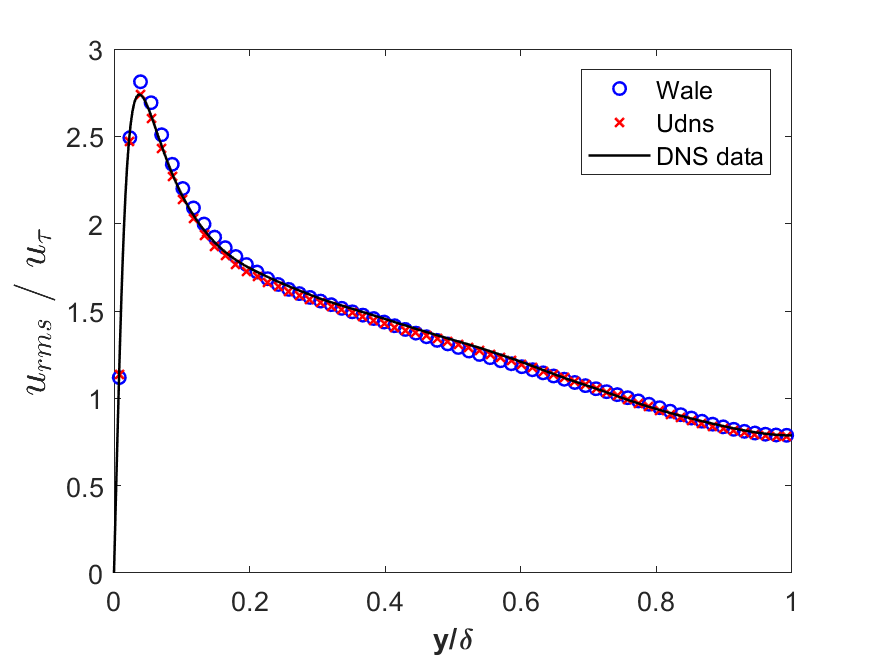
\includegraphics[width=6.7cm]{06_Resultsanddiscussion/figur/UDNSvsWale/urms_global_coords.png}}
\end{minipage}
%
\begin{minipage}[b]{0.5\textwidth}
\subfigure[wall coordinates]{
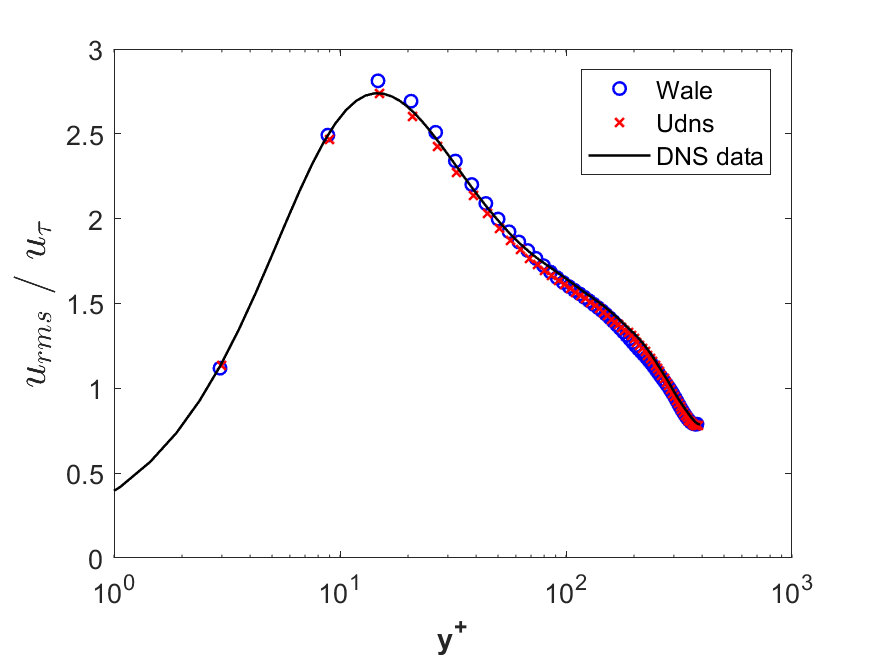
\includegraphics[width=6.7cm]{06_Resultsanddiscussion/figur/UDNSvsWale/urms_wall_coords.png}}
\end{minipage}
\caption{Rms profiles for the streamwise velocity fluctuation normalised by $u_\tau$}
\label{urms udns vs wale}
\end{figure} 
%

Fig. (\ref{vrms udns vs wale}) shows the $v_{rms}$ profile of UDNS and WALE with each other  and also with the profile of the DNS data. The comparison of the WALE and the UDNS profile shows that the WALE model dampens out the wall normal velocity fluctuations. This damping effect is present till $y^+ = 100$ and after that the profiles are in good agreement with each other. The peak value is underpredicted and the location of the peak value is overpredicted by both the UDNS and WALE profiles in comparison to the DNS data. 
%
\begin{figure}[h!]
\begin{minipage}[b]{0.5\textwidth}
\subfigure[global coordinates]{
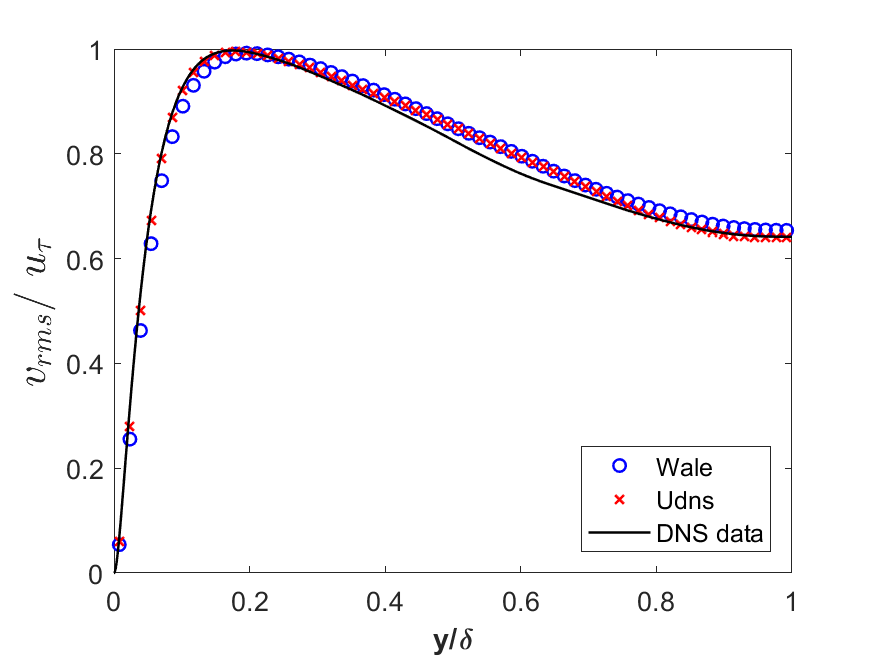
\includegraphics[width=6.7cm]{06_Resultsanddiscussion/figur/UDNSvsWale/vrms_global_coords.png}}
\end{minipage}
%
\begin{minipage}[b]{0.5\textwidth}
\subfigure[wall coordinates]{
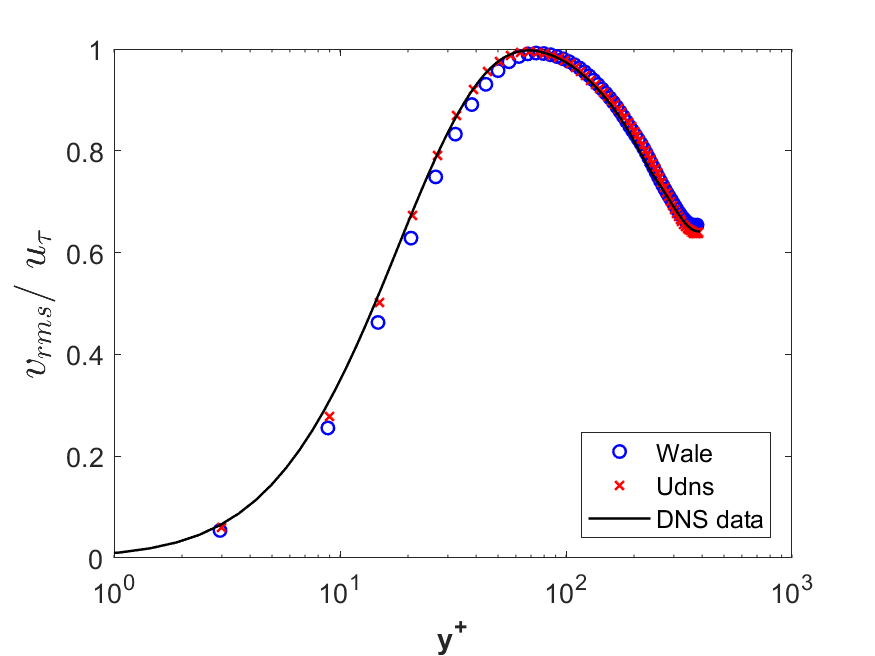
\includegraphics[width=6.7cm]{06_Resultsanddiscussion/figur/UDNSvsWale/vrms_wall_coords.png}}
\end{minipage}
\caption{Rms profiles for the wall-normal velocity fluctuation normalised by $u_\tau$}
\label{vrms udns vs wale}
\end{figure} 
%

Fig. (\ref{wrms udns vs wale}) shows the $w_{rms}$ profile of UDNS and WALE with each other  and also with the profile of the DNS data. The WALE model dampens out the spanwise velocity fluctuations in comparison to the UDNS profile. This effect is present till $y^+ = 100$ and after that the profiles are in good agreement. Both profiles overpredict the peak value and the location of the peak value in comparison to the DNS data. This can be seen by the slightly leftwards tilted velocity profiles.
%
\begin{figure}[h!]
\begin{minipage}[b]{0.5\textwidth}
\subfigure[global coordinates]{
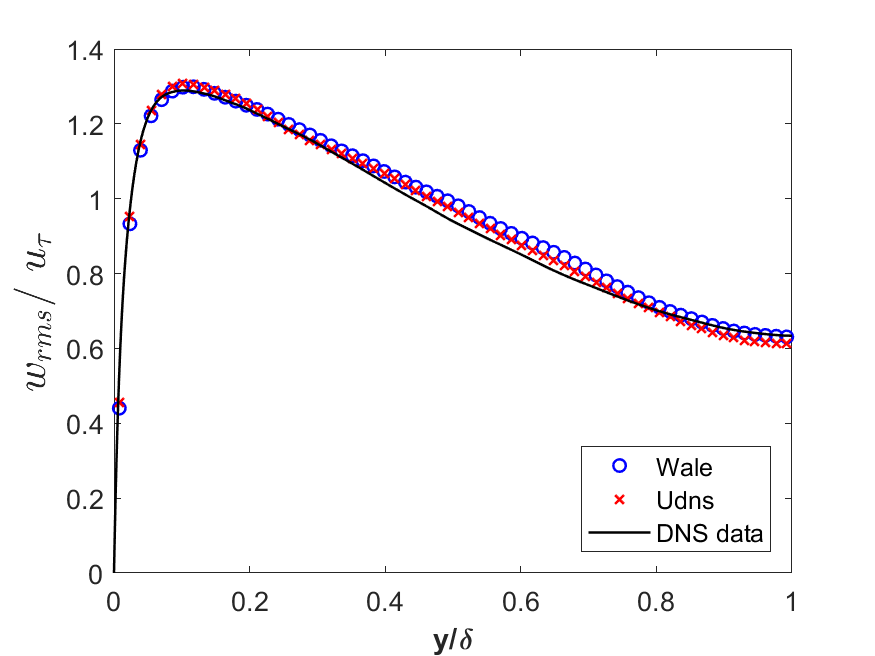
\includegraphics[width=6.7cm]{06_Resultsanddiscussion/figur/UDNSvsWale/wrms_global_coords.png}}
\end{minipage}
%
\begin{minipage}[b]{0.5\textwidth}
\subfigure[wall coordinates]{
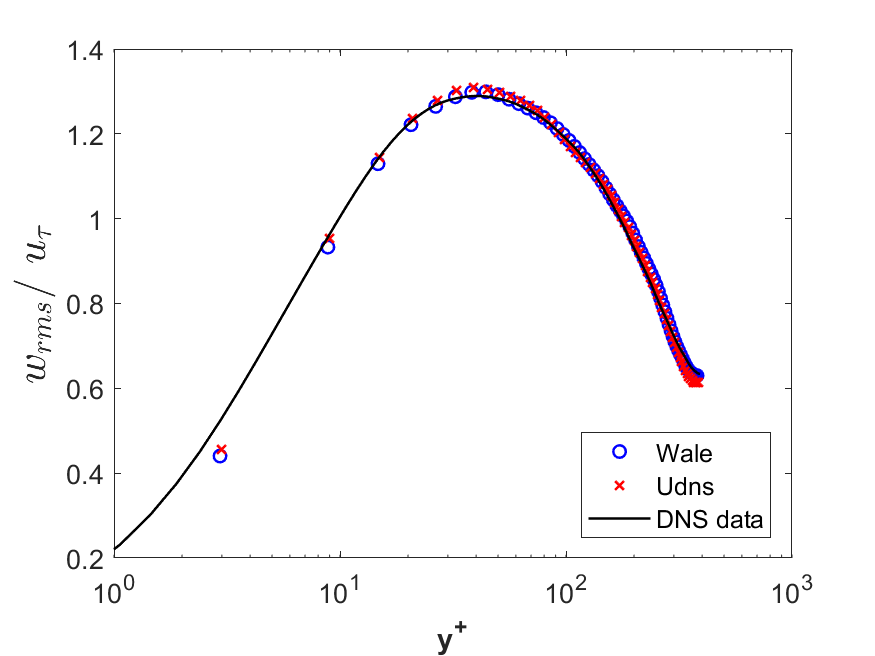
\includegraphics[width=6.7cm]{06_Resultsanddiscussion/figur/UDNSvsWale/wrms_wall_coords.png}}
\end{minipage}
\caption{Rms profiles for the spanwise velocity fluctuation normalised by $u_\tau$}
\label{wrms udns vs wale}
\end{figure} 
%

Thus, from the comparison of the rms velocity profiles for all components with the UDNS and WALE it is observed that the mean velocity profile for the WALE model overpredicts the UDNS profile $y^+ = 100$ and then they are in good agreement. Also does the WALE profile overpredicts the peak value in comparison to that of the DNS data. With the other two fluctuating velocity components the WALE model dampens out the respective fluctuations till around $y^+ = 100$ in comparison to the UDNS profile. For wall-normal velocity fluctuation both profiles underpredict the peak value and for the spanwise velocity fluctuation both profiles overpredict the peak value. From the comparison of the WALE and the UDNS profiles it seems that the $\nu_t$ has a minimal effect.

\subsubsection{Turbulent shear stress}
Fig. (\ref{uvrms udns vs wale}) shows the comparison of the turbulent shear stress profiles of WALE and UDNS with each other as well as with the DNS data. WALE and UDNS profiles are in good agreement with each other except for the region between $y^+ = 30$ to $y^+ = 170$ where the UDNS profile underpredicts the WALE and the DNS data profiles. After $y^+ = 170$ the profile fluctuates about the DNS data like a mean. Thus this underprediction can be attributed to the insufficinet averaging for that case. Overall profile of WALE is in good agreement with the DNS data. 
%
\begin{figure}[h!]
\begin{minipage}[b]{0.5\textwidth}
\subfigure[global coordinates]{
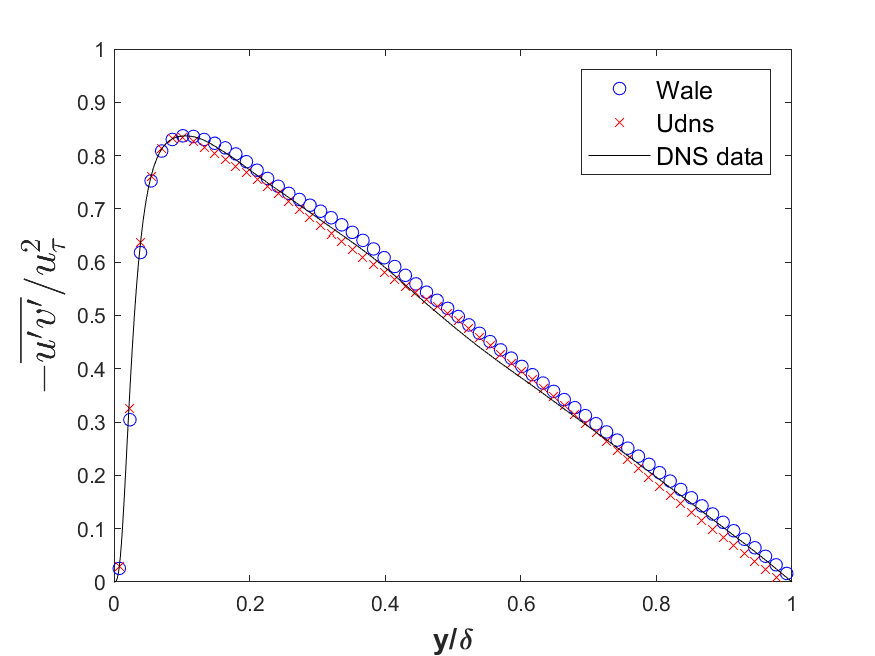
\includegraphics[width=6.7cm]{06_Resultsanddiscussion/figur/UDNSvsWale/uv_rms_global_coords.png}}
\end{minipage}
%
\begin{minipage}[b]{0.5\textwidth}
\subfigure[wall coordinates]{
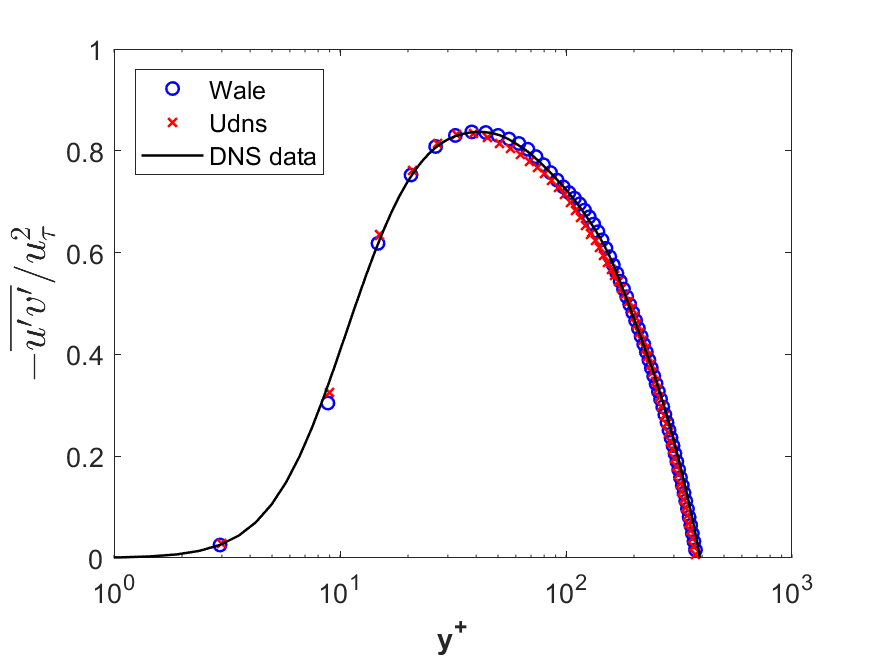
\includegraphics[width=6.7cm]{06_Resultsanddiscussion/figur/UDNSvsWale/uv_rms_wall_coords.png}}
\end{minipage}
\caption{Turbulent shear stress profiles normalised by $u_\tau^2$}
\label{uvrms udns vs wale}
\end{figure} 
%

\subsection{Comparison UDNS and WALE, $Re_\tau = 550$}
The comparison of the UDNS and the WALE model profiles for $Re_\tau = 395$ did not show any noteworthy difference. A slight difference, less than $1\%$, is observed in the mean velocity profile and the Reynolds stress profiles. The initial assumption was that $\nu_t$ is not sufficient enough to create a noticeable difference. Thus it was decided to perform a simulation with the higher Reynolds number, $Re_\tau = 550$. The DNS results of~\cite{lee:moser:15} , for $Re_\tau = 550$, will be used as a reference for the comparison. The DNS data for the comparison can be obtained from the database of turbulent channel flow~\cite{channeldata:99}.

The main purpose for performing this simulation is to have some noticeable difference between the WALE and the UDNS results with the increased Reynolds number. The domain size was same as that used for the investigation with $Re_\tau = 395$. The simulation has been performed on the Mesh 1 resolution. The table (\ref{Physical quantities 550}) shows the values of the physical quantities in both S.I and LB units. The Ma number of the flow $Ma_{act} = 0.002915452$ is very small and for the reason mentioned in subsection (\ref{Mach reference}) the Ma number is artificially increased to $Ma_{art} = 0.173205081$. The table (Solver settings 550) shows the solver settings.\\

%
\begin{table}[!h]
\centering
\begin{tabular}{c|c|c}
%\hline
$ Physical\ quantity$ & $ S.I\ Units$ & $LB\ units$  \\
\hline
%
Half channel height, $\de$ & $1.0\ m$ & $32\Delta x$\\
\hline
%
Friction velocity, $u_\tau$ & $0.0543496\ m/s$ & $-$ \\
\hline
%
Bulk velocity, $U_b$ & $1\ m/s$ & $0.1 \Delta x/ \Delta t$ \\
\hline
%
Kinematic Viscosity, $\nu$ & $0.0001\ m^2/s$ & $0.00032 \Delta x^2 / \Delta t$\\
\hline
%
\end{tabular}
\caption{Physical quantities, $Re_\tau = 550$}
\label{Physical quantities 550}
\end{table}
%
%
\begin{table}[h!]
\begin{center}
\begin{tabular}{ |p{2cm}|p{1.5cm}|p{2cm}|  } 
\hline
 &$\sim time$ & Mesh1 \\
  \hline
  \multirow{3}{6em}{Flow developing stage} & $t\ [s]$ & 1562.5  \\
  & $tu_\tau/\delta$ & 84 \\ 
  & $tU_b/\delta$ & 1562.5 \\ 
  \hline
  \multirow{3}{6em}{Averaging stage} & $t [s]$ & 9062.5 \\
  & $tu_\tau/\delta$ & 492.54  \\ 
  & $tU_b/\delta$ & 9062.5 \\ 
  \hline
\end{tabular}
\end{center}
\caption{Solver settings, $Re_\tau = 550$}
\label{Solver settings 550}
\end{table}
%
\textbf{Mean velocity profile}
%
\begin{figure}[h!]
\begin{minipage}[b]{0.5\textwidth}
\subfigure[global coordinates]{
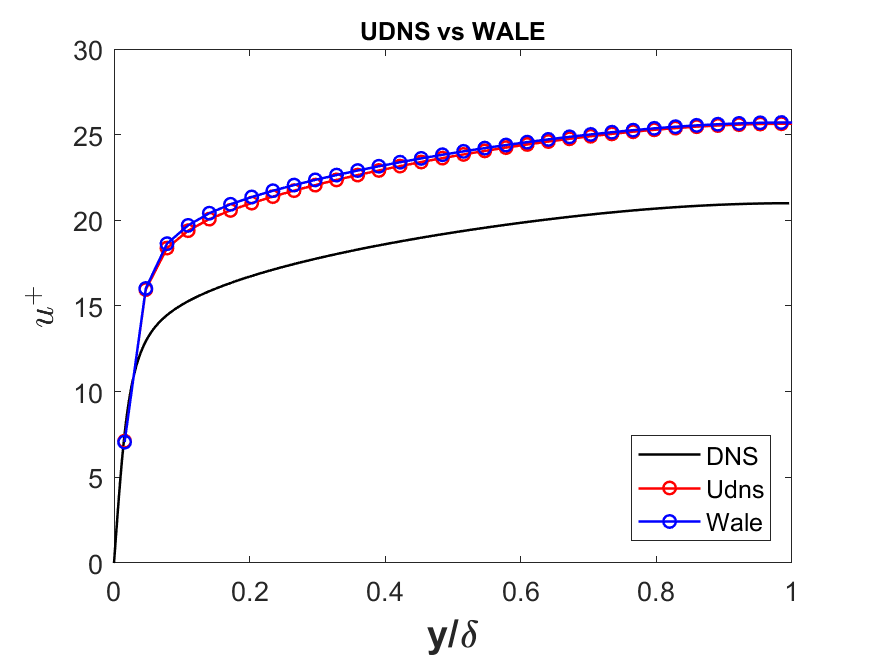
\includegraphics[width=6.7cm]{06_Resultsanddiscussion/figur/Re_tau_550/Profile_global_coords.png}}
\end{minipage}
%
\begin{minipage}[b]{0.5\textwidth}
\subfigure[local coordinates]{
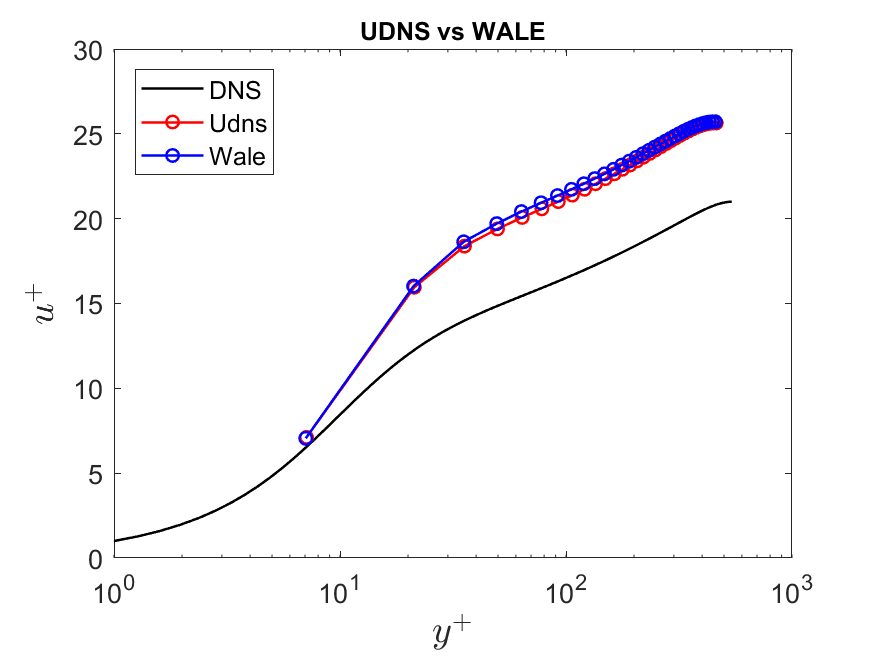
\includegraphics[width=6.7cm]{06_Resultsanddiscussion/figur/Re_tau_550/Profile_wall_coords_theo_comp.png}}
\end{minipage}
\caption{Mean velocity profiles, $Re_\tau = 550$}
\label{mean profiles 550}
\end{figure} 
%
The resulting quantities for UDNS and WALE have listed in the table (\ref{Global quantities results 550}) along with the target values.
%
\begin{table}[h!]
\begin{center}
\begin{tabular}{ p{3cm}|p{1.5cm}p{1.5cm}p{1.5cm}  } 
\hline
Physical quantity & WALE & UDNS & Target \\
  \hline
  \multirow{1}{6em}{$u_\tau,\ m/s$}  & 0.0451 & 0.0455 & 0.0550\\
  \hline
  \multirow{1}{6em}{$Re_\tau$} & 451 & 455 & 550\\
  \hline
%  \multirow{1}{6em}{$U_c,\ m/s$} & 0.1562 & 0.1557 & 0.1547 & 0.1591\\
%  \hline
\end{tabular}
\end{center}
\caption{Comparison of the computed physical quantities using WALE model \& UDNS $Re_\tau = 550$}
\label{Global quantities results 550}
\end{table}
%
Fig. (\ref{mean profiles 550}) shows the mean velocity profiles of UDNS and WALE compared with each other as well as with the DNS results. The profiles for UDNS and the WALE model overpredict the DNS profiles significantly. Noticeable difference is not seen between the UDNS and WALE profiles. Thus increasing the Reynolds number is also not helpful to see the $\nu_t$ influencing the WALE mean velocity profiles. Since no positive outcome is obtained from these profiles, the profiles for the turbulence intensity and the Reynolds stress will not be shown or discussed.

\subsection{Conclusion and Outlook}